% ecexpo_presentation.tex

% Copyright 2019 Clara Eleonore Pavillet

% Author: Clara Eleonore Pavillet
% Description: This is an unofficial Oxford University Beamer Template I made from scratch. Feel free to use it, modify it, share it.
% Version: 1.0

\documentclass{beamer}
\usepackage{import} % for some reason, this doesn't work when called in sty file
% Load Packages
\usepackage[utf8]{inputenc}
\usepackage{xcolor}
\usepackage{tikz}
\usetikzlibrary{positioning,calc}
\usepackage{graphicx}
\usepackage{hyperref}
\usepackage{amsmath}
\usepackage{listings}
\usepackage{fontawesome}

% Define Commands
\newcommand*{\ClipSep}{0.06cm} %To adjust footer logo
\newcommand{\E}{\mathrm{e}\,} %\def\I{e} % used to defined e for exp(x), see later what it should be
\newcommand{\ud}{\mathrm{d}}
\lstset{numbers=left, numberstyle=\tiny, stepnumber=1,firstnumber=1,breaklines=true,
    numbersep=5pt,language=Python,
    stringstyle=\ttfamily,
    basicstyle=\footnotesize, 
    showstringspaces=false
}

\usepackage{lecture_notes}
\usepackage{bibentry}
\usepackage[utf8]{inputenc}
\usepackage[T1]{fontenc}

\graphicspath{ {../images/} }

\nobibliography*
% \usepackage[perpage]{footmisc}
\usetheme{oxonian}

\newcommand{\fignocap}[2]{
	\begin{figure}[!hbtp]
	    \centering
		\includegraphics[width=#1\linewidth]{#2}
	\end{figure}
}

\newcommand{\subfignocap}[5]{
  \begin{figure}[!hbtp]
      \centering
    \subfigure{\includegraphics[width=#1\linewidth]{#2}}
    \hspace{#5}%
    \subfigure{\includegraphics[width=#3\linewidth]{#4}}
  \end{figure}
}

% vec
\renewcommand{\vec}[1]{\mathbf{#1}}

% MSE
\newcommand{\mse}[1]{\text{MSE}\left({#1}\right)}

% https://tex.stackexchange.com/questions/434931/reorder-note-field-at-the-end-of-the-reference
% \DeclareSourcemap{
%   \maps[datatype=bibtex]{
%     \map[overwrite=false]{
%       \step[fieldsource=note]
%       \step[fieldset=addendum, origfieldval, final]
%       \step[fieldset=note, null]
%     }
%   }
% }

\title{Efficient Deep Learning for Massive MIMO Channel State Estimation}
\titlegraphic{
\includegraphics[width=3cm]{Theme/Logos/DavisLogoV1.png}}
\author{\small{Mason del Rosario}}
\institute{Doctoral Qualifying Examination}
\date{May 2021} %\today

\begin{document}
% \bibliographystyle{ieeetr}
% \nobibliography*{refs}


{\setbeamertemplate{footline}{} 
\frame{\titlepage}}

\section*{Outline}\begin{frame}{Outline}\tableofcontents\end{frame}

\section{Background}
   %  \begin{frame}[plain]
   %    \vfill
   %    \centering
   %    \begin{beamercolorbox}[sep=8pt,center,shadow=true,rounded=true]{title}
   %      \usebeamerfont{title}\insertsectionhead\par%
   %      \color{davisblue}\noindent\rule{10cm}{1pt} \\
   %      % \LARGE{\faFileTextO}
   %    \end{beamercolorbox}
   %    \vfill
  	% \end{frame}

  % Background section frame 
  \begin{frame}[plain]
    \vfill
    \centering
    \begin{beamercolorbox}[sep=8pt,center,shadow=true,rounded=true]{Background}
      \usebeamerfont{title}\insertsectionhead\par%
      \color{davisblue}\noindent\rule{10cm}{1pt} \\
      % \LARGE{\faFileTextO}
    \end{beamercolorbox}
    \vfill
  \end{frame}

\subsection{Role of CSI in MIMO}
  \nofoot{
	\begin{frame}{Why MIMO?}
		Massive MIMO is a key enabling technology for future wireless communications networks.
		\begin{itemize}
			\item 5G, Ultra-Dense Networks, IoT
		\end{itemize}
		\pause
		The efficacy of MIMO depends on accurate \emph{Channel State Information (CSI)}.
    \blfootnote{S. Marek, ``Sprint Spent \$1B on Massive MIMO for Its 5G Network in Q2," \emph{SDxCentral}, \url{https://www.sdxcentral.com/articles/news/sprint-spent-1b-on-massive-mimo-for-its-5g-network-in-q2/2018/06/}. Accessed: Feb 22, 2020.}
	\end{frame}
  }

	\begin{frame}{MIMO and CSI}
		Massive MIMO uses numerous antennas to endow transceivers with spatial diversity.
		\fignocap{0.8}{mimo-nopre.PNG}
	\end{frame}

	\begin{frame}{MIMO and CSI}
		The fading coefficients between each set of Tx/Rx antennas constitute \textbf{Channel State Information (CSI)}, $\mathbf{H}$. For $n_T$, $n_R$ antennas,
		\begin{align*}
			\mathbf{H}&=\begin{bmatrix}
							h_{1,1} & h_{1,2} & \dots  & h_{1,n_T} \\
							h_{2,1} & h_{2,2} & \dots  & h_{2,n_T} \\
							\vdots	& \vdots  & \vdots & \vdots    \\
							h_{n_{R},1} & h_{n_{R},2} & \dots  & h_{n_{R},n_T} \\
						\end{bmatrix}
		\end{align*}
	\end{frame}

	\begin{frame}{MIMO and Perfect CSI}
		\textbf{Perfect CSI} (i.e., exact knowledge of the channel, $\mathbf{H}$) allows us to maximize the power of the received symbol by precoding.
		\fignocap{0.8}{mimo-pre.PNG}
	\end{frame}

	\begin{frame}{MIMO and CSI Estimation}
		However, transmitting $\mathbf{H}$ is costly. Instead, generate \textbf{CSI Estimates}, $\hat{\mathbf{H}}$, based on \textbf{compressed feedback}.\\
		\fignocap{0.8}{mimo-feed.PNG}
    \textbf{Goal}: Find low-dimensional representation, feed back to transmitter for recovery of $\hat{\mathbf{H}}$ which is an accurate approximation of $\mathbf{H}$ in MSE sense. % add something about need fro compression
	\end{frame}

\section{CSI Estimation}
  % \subsection{Conventional Methods}
  %   \begin{frame}{Compressed Sensing}
  %     Find a low-dimensional representation of data by a linear transform, i.e.
  %     \begin{align*}
  %       \vec{y}&=\Psi\vec{h} \\ %https://www.sciencedirect.com/topics/computer-science/compressed-sensing 
  %       \vec{h}&=\Phi\vec{y}
  %     \end{align*}
  %     where $\vec{h}$ is a vectorized version of CSI measurements at UE.
  %     % Reference for equation? Claims
  %     Takes advantage of \emph{sparsity} of CSI matrices. \pause

  %     \textbf{Problems:} Strong sparsity assumptions, not necessarily true in real-world data. Iterative algorithms = computationally expensive.
  %     % [1] ???
  %     % [2] https://www.sciencedirect.com/science/article/pii/B9780123849885000450 
    % \end{frame}
  \subsection{Convolutional Neural Networks}

    \nofoot{
    \begin{frame}{Convolutional Neural Networks (CNNs)}
      \begin{itemize}
        \item CNNs = state-of-the art performance in image processing applications
        \item Capable of extracting features from 2D, grid-like data 
      \end{itemize}
      \fignocap{0.35}{filt1.JPEG}
      \pause
      \begin{itemize}
        \item \textbf{Recently, CNNs applied to CSI estimation}
      \end{itemize}
      \blfootnote{A. Karpathy, ``Visualizing What ConvNets Learn,"  \url{http://cs231n.github.io/understanding-cnn/}. Accessed: Feb 24, 2020.}
    \end{frame}
    }

    \nofoot{
    \begin{frame}{CsiNet}
      \begin{itemize}
        \item CNN-based autoencoder for learned CSI compression and feedback \cite{ref:csinet}
        % \item Expanded their work to use Recurrent Neural Networks \cite{ref:Wang2019CsiNetLSTM}
      \end{itemize}
      \fignocap{0.9}{csinet-fig.PNG}
      % [3] CsiNet paper
      % [4] CsiNet-LSTM paper
      \blfootnote{\bibentry{ref:csinet}}
    \end{frame}
    }

    % \nofoot{
    % \begin{frame}{Domain Knowledge}
    %     \fignocap{0.55}{conway-venn.PNG}
    %   % [5] Conway blog post
    %   \blfootnote{D. Conway, ``Data Science Venn Diagram," \url{http://drewconway.com/zia/2013/3/26/the-data-science-venn-diagram}. Accessed: Feb 20, 2020}
    % \end{frame}
    % }


\section{Spherical Normalization}

  % Spherical Normalization section frame 
  \begin{frame}[plain]
    \vfill
    \centering
    \begin{beamercolorbox}[sep=8pt,center,shadow=true,rounded=true]{Spherical Normalization}
      \usebeamerfont{title}\insertsectionhead\par%
      \color{davisblue}\noindent\rule{10cm}{1pt} \\
      % \vspace{8pt}
      \footnotesize{Power-based normalization for improved CSI reconstruction accuracy.}
      % \LARGE{\faFileTextO}
    \end{beamercolorbox}
    \vfill
  \end{frame}

  \begin{frame}{CsiNet: Minmax Normalization}
    Most works perform \textbf{minmax scaling} -- Take the extrema ($\mathbf H_{\text{min}}, \mathbf H_{\text{max}}$) of the real and imaginary channels, 
    \begin{align*}
      \mathbf H_{n,\text{minmax}}(i,j) &= \frac{\mathbf H_n(i,j)-\mathbf H_{\text{min}}}{\mathbf H_{\text{max}}-\mathbf H_{\text{min}}} \in [0,1],
    \end{align*}
    for $n \in [1,\dots,N]$ given $N$ samples and $i,j$ indexing rows/columns of CSI matrices.
  \end{frame}

    \begin{frame}{CsiNet: Minmax Normalization}
      % \footnotesize{
      % \begin{figure}[!hbtp] \centering 
      %   \subfigure[COST2100 Indoor - real/imaginary channels ($N=99000$)] {\label{fig:cost2100_minmax_range} 
      %   % 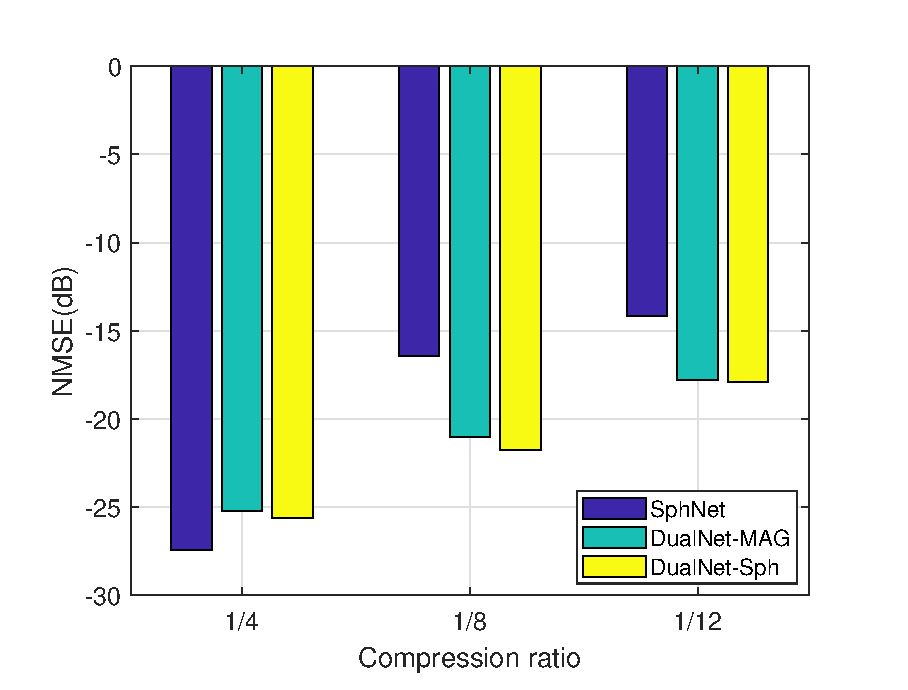
\includegraphics[width=0.46\textwidth]{images/nmse_indoor_mag.eps}
      %   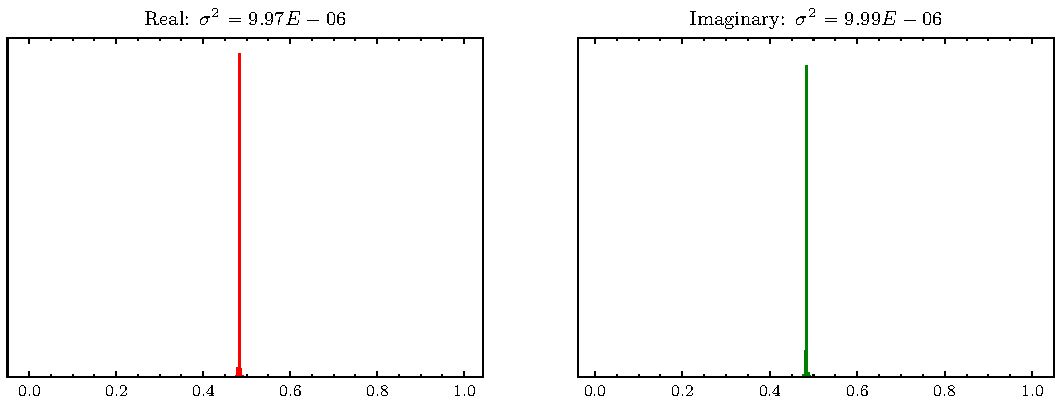
\includegraphics[width=0.47\textwidth]{cost2100_indoor_dist.pdf}
      %   } 
      %   \subfigure[ImageNet - RGB channels ($N=50000$)] { \label{fig:imagenet_minmax_range} 
      %   % 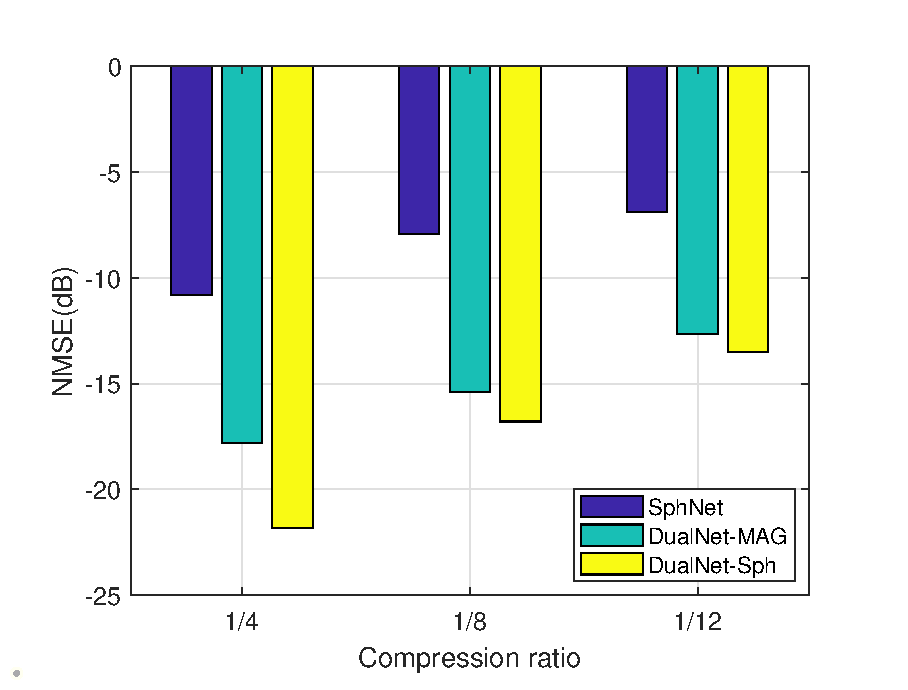
\includegraphics[width=0.46\textwidth]{images/nmse_outdoor_mag.eps} 
      %   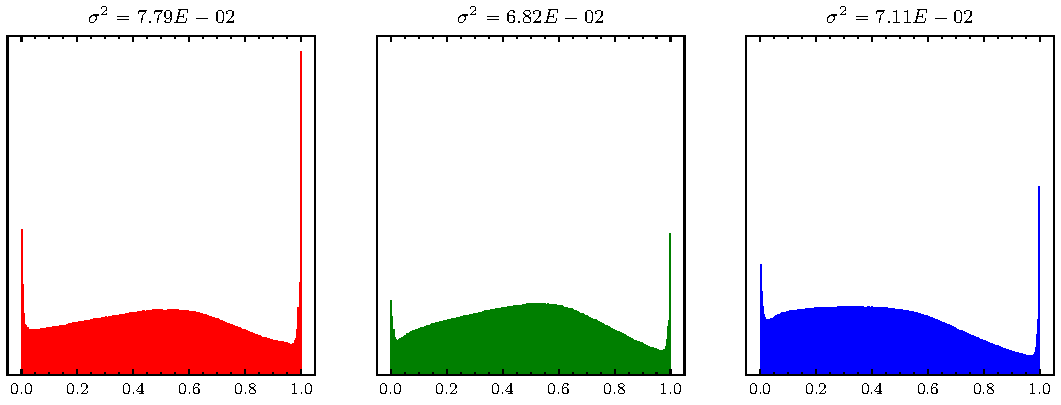
\includegraphics[width=0.47\textwidth]{imagenet_rgb_dist.pdf}
      %   } 
      %   \caption{Distribution and variance of minmax-normalized channels for two datasets.} 
      %   \label{fig:minmax} \vspace*{-2mm}
      % \end{figure}
      %   }
      \begin{figure}[htb]
        \centering
        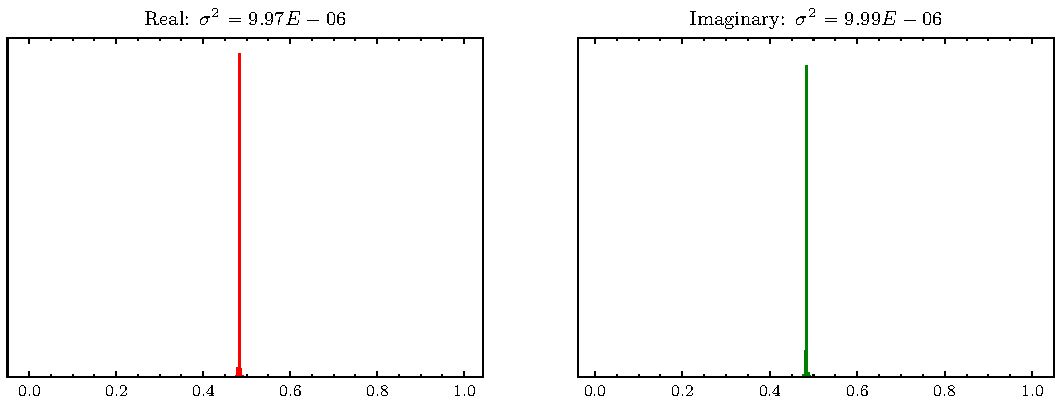
\includegraphics[width=.9\textwidth]{cost2100_indoor_dist.pdf}
        \medskip
        \caption{Distribution and variance of minmax-normalized COST2100 real/imaginary channels ($N=99000$) images.}
        \label{fig:cost_indoor_dist}
      \end{figure}
    \end{frame}

    \begin{frame}{ImageNet: Minmax Normalization}
      \begin{figure}[htb]
        \centering
        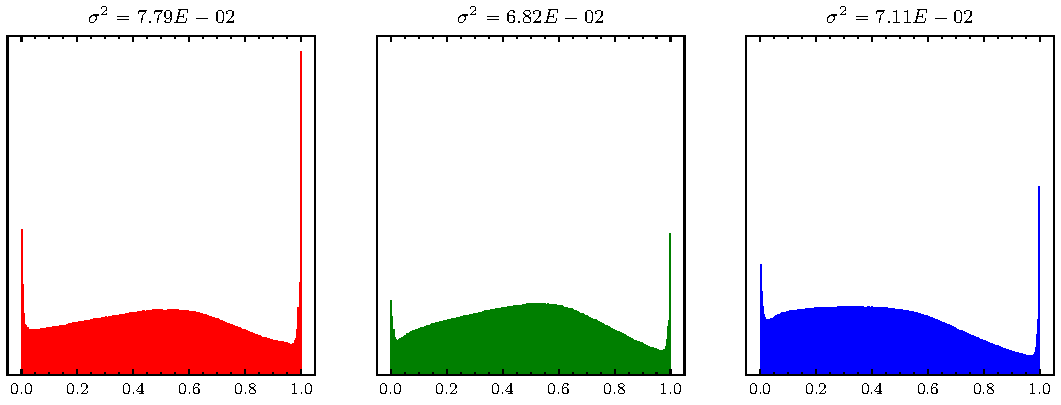
\includegraphics[width=.9\textwidth]{imagenet_rgb_dist.pdf}
        \medskip
        \caption{Distribution and variance of minmax-normalized ImageNet color channels ($N=50000$) images.}
        \label{fig:imagenet_dist}
      \end{figure}
    \end{frame}

  % \nofoot{
  % \subsection{Bi-directional Reciprocity}
  % \begin{frame}{Bi-directional Reciprocity}
  %   \begin{columns}[T] % align columns
  %   \begin{column}{.48\textwidth}
  %   \begin{itemize}
  %     \item Goal = estimate downlink CSI
  %     \item In conventional CSI estimation for FDD, uplink is typically not used to estimate downlink
  %     \item With CNNs, can leverage correlation between uplink/downlink \cite{ref:dualnet}
  %   \end{itemize}
  %   \end{column}%
  %   \hfill%
  %   \begin{column}{.5\textwidth}
  %     \fignocap{0.9}{images/corr-fig.PNG}
  %   \end{column}%
  %   \end{columns}
  %   \blfootnote{\bibentry{ref:dualnet}}
  % \end{frame}
  % }

  % \begin{frame}{Bi-directional Reciprocity}
  %   \fignocap{1.0}{images/dualnet-fig.PNG}
  % \end{frame}

\subsection{Spherical Normalization}
  \begin{frame}{Spherical Normalization}
    \textbf{Spherical normalization} -- scale each channel sample by its power,
    % TODO: Does this make sense? "For CSI matrices, we could choose to scale each element by it's mean and by the inverse covariance matrix."
    \begin{align}
      \mathbf{\check H}_d^n &= \frac{\mathbf H_d^n}{\|\mathbf H_d^n\|_2}. \label{eq:sph-intro}
    \end{align}
    After applying (\ref{eq:sph-intro}) to each sample, minmax scaling is applied to the entire dataset.
  \end{frame}

  \begin{frame}{SphNet: Spherical Normalization}
    The resulting dataset under spherical normalization can exhibits a larger variance than the same dataset under minmax scaling. 
    \begin{figure}[htb]
      \centering
      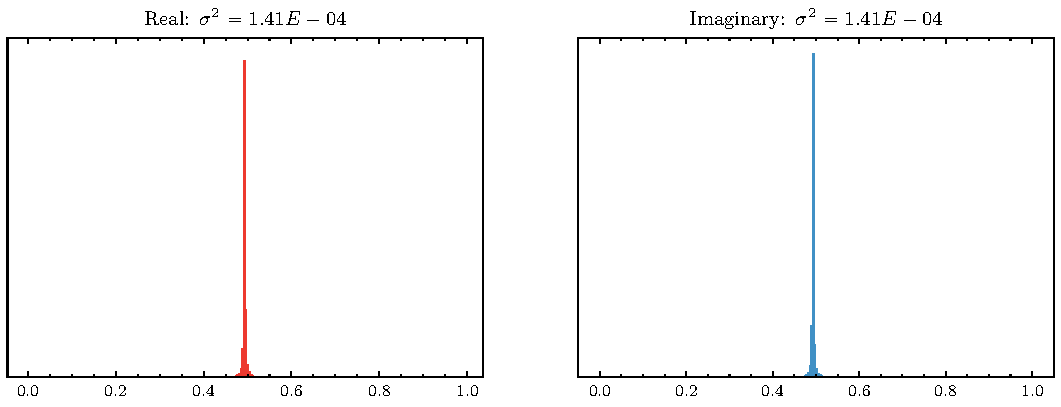
\includegraphics[width=.9\textwidth]{cost2100_indoor_sph_dist.pdf}
      % \medskip
      \caption{Distribution and variance of COST2100 real/imaginary channels under spherical normalization ($N=99000$) images.}
      \label{fig:cost_indoor_sph_dist}
    \end{figure}
  \end{frame}

  \begin{frame}{MSE/NMSE equivalence}
    \footnotesize{
    Under spherical normalization, MSE loss becomes equivalent to NMSE. Recall the definitions,
    \begin{align*} 
      \text{MSE}=\frac 1N \sum_{k=1}^N\Arrowvert\mathbf H_k - \hat{\mathbf H}_k\Arrowvert^2,\quad \text{NMSE} =\frac 1N \sum_{k=1}^N\frac{\Arrowvert\mathbf H_k - \hat{\mathbf H}_k\Arrowvert^2}{\Arrowvert\mathbf H_k\Arrowvert^2} \\        
    \end{align*}
    The MSE of the spherically normalized estimator is equivalent to the NMSE of the regular estimator, i.e.
    \begin{align*}
      \text{MSE}_{\text{Sph}} &= \frac 1N \sum_{k=1}^N\Arrowvert\check{\mathbf H}_k - \hat{\check{\mathbf H}}_k\Arrowvert^2 \\
      &= \frac 1N \sum_{k=1}^N\left\Arrowvert \frac{\mathbf H_k}{\Arrowvert\mathbf H_k\Arrowvert^2} - \frac{\hat{\mathbf H}_k}{\Arrowvert\mathbf H_k\Arrowvert^2}\right\Arrowvert^2 \\
      &= \frac 1N \sum_{k=1}^N\frac{\Arrowvert\mathbf H_k - \hat{\mathbf H}_k\Arrowvert^2}{\Arrowvert\mathbf H_k\Arrowvert^2} \; \Box.
      % &= \text{NMSE} \; \Box
    \end{align*}
    }
\end{frame}
  % \begin{frame}{Spherical Normalization}
  %   CSI matrices are sparse in 2D (angular) delay domain.
  %   \begin{figure}[ht]
  %   \centering
  %   \incfig{csi-reshape}{0.75\columnwidth}
  %   % \caption{Pre-normalized data.}
  %   % \label{fig:csi-pre-norm}
  %   \end{figure}
  % \end{frame}

  % \begin{frame}{Spherical Normalization}
  %   CSI matrices are sparse in 2D (angular) delay domain.
  %   \begin{figure}[ht]
  %   \centering
  %   \incfig{csi-pre-norm}{0.75\columnwidth}
  %   % \caption{Pre-normalized data.}
  %   % \label{fig:csi-pre-norm}
  %   \end{figure}
  % \end{frame}

  % \begin{frame}{Spherical Normalization}
  %   Naive normalization of dataset, $\vec{H}$: cast all values to range [0,1] by scaling all entries by $\text{max}\left(\vec{H}\right)-\text{min}\left(\vec{H}\right)$.
  %   \begin{figure}[ht]
  %   \centering
  %   \incfig{csi-naive-norm}{0.75\columnwidth}
  %   % \caption{Pre-normalized data.}
  %   % \label{fig:csi-pre-norm}
  %   \end{figure}
  %   \pause
  %   \begin{itemize}
  %   \item Low-magnitude entries have less influence in updates during training.
  %   \end{itemize}
  % \end{frame}

  % \begin{frame}{Spherical Normalization}
  %   \textbf{Solution: Spherical normalization}. Scale each entry by sample power, $||\mathbf{H}_k||$. % Training data, $\check{\vec{H}}$, become
  %   \begin{figure}[ht]
  %   \centering
  %   \incfig{csi-sph-norm}{0.75\columnwidth}
  %   % \caption{Pre-normalized data.}
  %   % \label{fig:csi-pre-norm}
  %   \end{figure}
  %   \pause
  %   \begin{itemize}
  %   \item Low-magnitude entries maintain influence in updates during training.
  %   \end{itemize}
  %   % \begin{align*}
  %   %   \check{\vec{H}}^k = \frac{\vec{H}^k}{||\vec{H}^k||} 
  %   % \end{align*}
  %   % where $k$ denotes the $k-$th sample in the dataset. Compare with min-max training data, $\bar{\vec{H}}$,
  %   % \begin{align*}
  %   %   \bar{\vec{H}}^k = \frac{\vec{H}^k}{\text{max}\left(\vec{H}\right)-\text{min}\left(\vec{H}\right)} 
  %   % \end{align*}
  % \end{frame}

  \begin{frame}{SphNet: Spherical Normalization}
    \fignocap{0.9}{sphnet-fig.PNG}
  \end{frame}



  % \nofoot{
  % \begin{frame}{Spherical Normalization: Results}
  %   \begin{figure}[!hbtp] \centering 
  %   \subfigure[Indoor] {\label{fignmse:a} 
  %   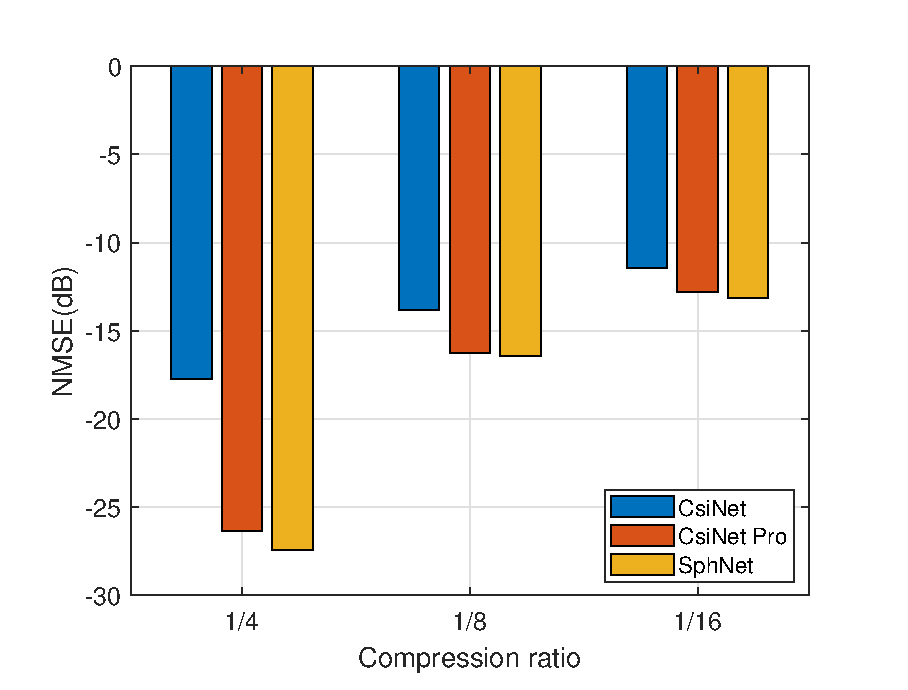
\includegraphics[width=0.46\textwidth]{images/nmse_indoor.eps}
  %   } 
  %   \subfigure[Outdoor] { \label{fignmse:b} 
  %   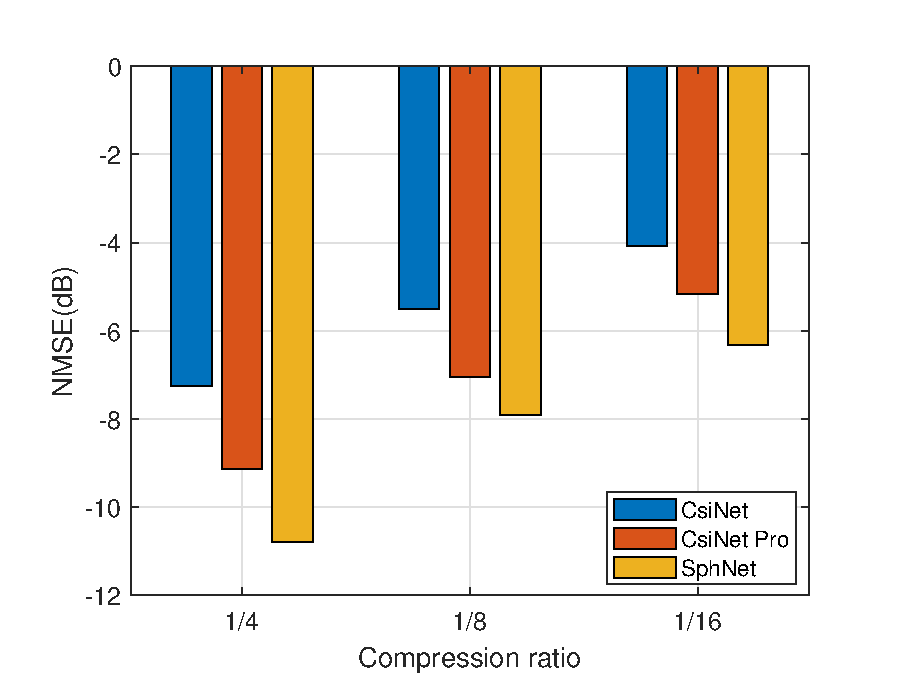
\includegraphics[width=0.46\textwidth]{images/nmse_outdoor.eps} 
  %   } 
  %   \caption{NMSE (lower is better) comparison in different compression ratios for downlink-based CSI feedback.\cite{ref:liu2020sphnet}} 
  %   \label{fignmse} \vspace*{-2mm}
  %   \end{figure}
  %   \blfootnote{\bibentry{ref:liu2020sphnet}}
  % \end{frame}
  % }

  \nofoot{
  % 2x2 matrix denoting different test configurations
  \begin{frame}{Experimental Setup: Models}
    \begin{figure}[!hbtp] \centering 
      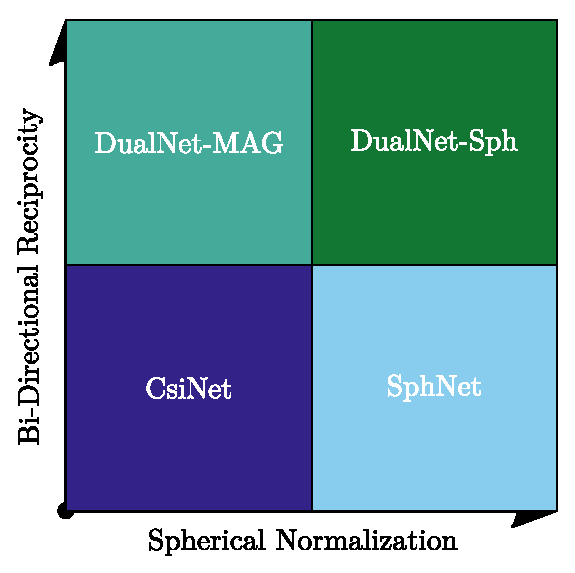
\includegraphics[width=0.47\textwidth]{00-experiment-grid.eps}
      \caption{Illustration of techniques used in different models.} 
      \label{fig:grid} \vspace*{-2mm}
    \end{figure}
    \blfootnote{\bibentry{ref:liu2020sphnet}}
  \end{frame}
  }

  \begin{frame}{Experimental Setup: Parameters}
    Two MIMO scenarios using COST 2100 model with 32 antennas at gNB and single UE (single antenna), 1024 subcarriers.
    \begin{enumerate}
        \item \textbf{Indoor} environment using 5.3GHz, 0.1 m/s UE mobility, square area of length $20$m
        \item \textbf{Outdoor} environment using 300MHz, 1 m/s UE mobility, square area of length $400$m
    \end{enumerate}
    \textbf{Dataset}: $10^5$ channel samples -- $70\% / 30\% $ training/test split. % vary compression ratio from $\frac{1}{4}$ to $\frac{1}{16}$

    \textbf{Hyperparameters}: Adam optimizer with learning rate $10^{-3},$ batch size $200,$ $1000$ epochs, MSE loss
    % For all experiments, we utilize $N_b=32$ antennas at the gNB and a single antenna at the UE. The gNB uses antennas arranged in a uniform linear array (ULA) with half-wavelength spacing. We use $N_f=1024$ subcarriers and truncate the delay-domain CSI matrix to include the first $Q_f=32$ rows. For each environment, we generate a large dataset of $10^5$ samples and split the dataset into $7\cdot 10^4$ and $3\cdot 10^4$ samples for training and validation sets, respectively. For training, we utilize Adam with a learning rate of $10^{-3}$ and a batch size of 200. Each network was trained for 1000 epochs using MSE (as Eq. (\ref{eq:mse})) as the loss function, and the figure of merit used to compare all networks was NMSE (as Eq. (\ref{NMSE})). All networks were trained for three different compression ratios, $\frac{1}{4}, \frac{1}{8},$ and $\frac{1}{16}$.
  \end{frame}

  \nofoot{
  \begin{frame}{Experimental Results}
    \begin{figure}[!hbtp] \centering 
      \subfigure[Indoor] {\label{fignmse_mag:a} 
      % 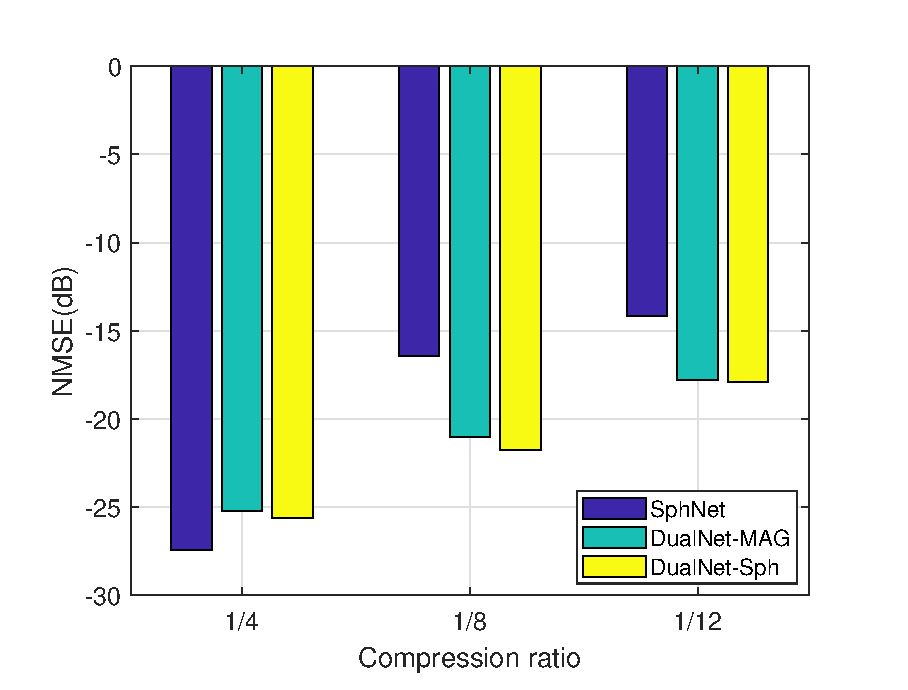
\includegraphics[width=0.46\textwidth]{images/nmse_indoor_mag.eps}
      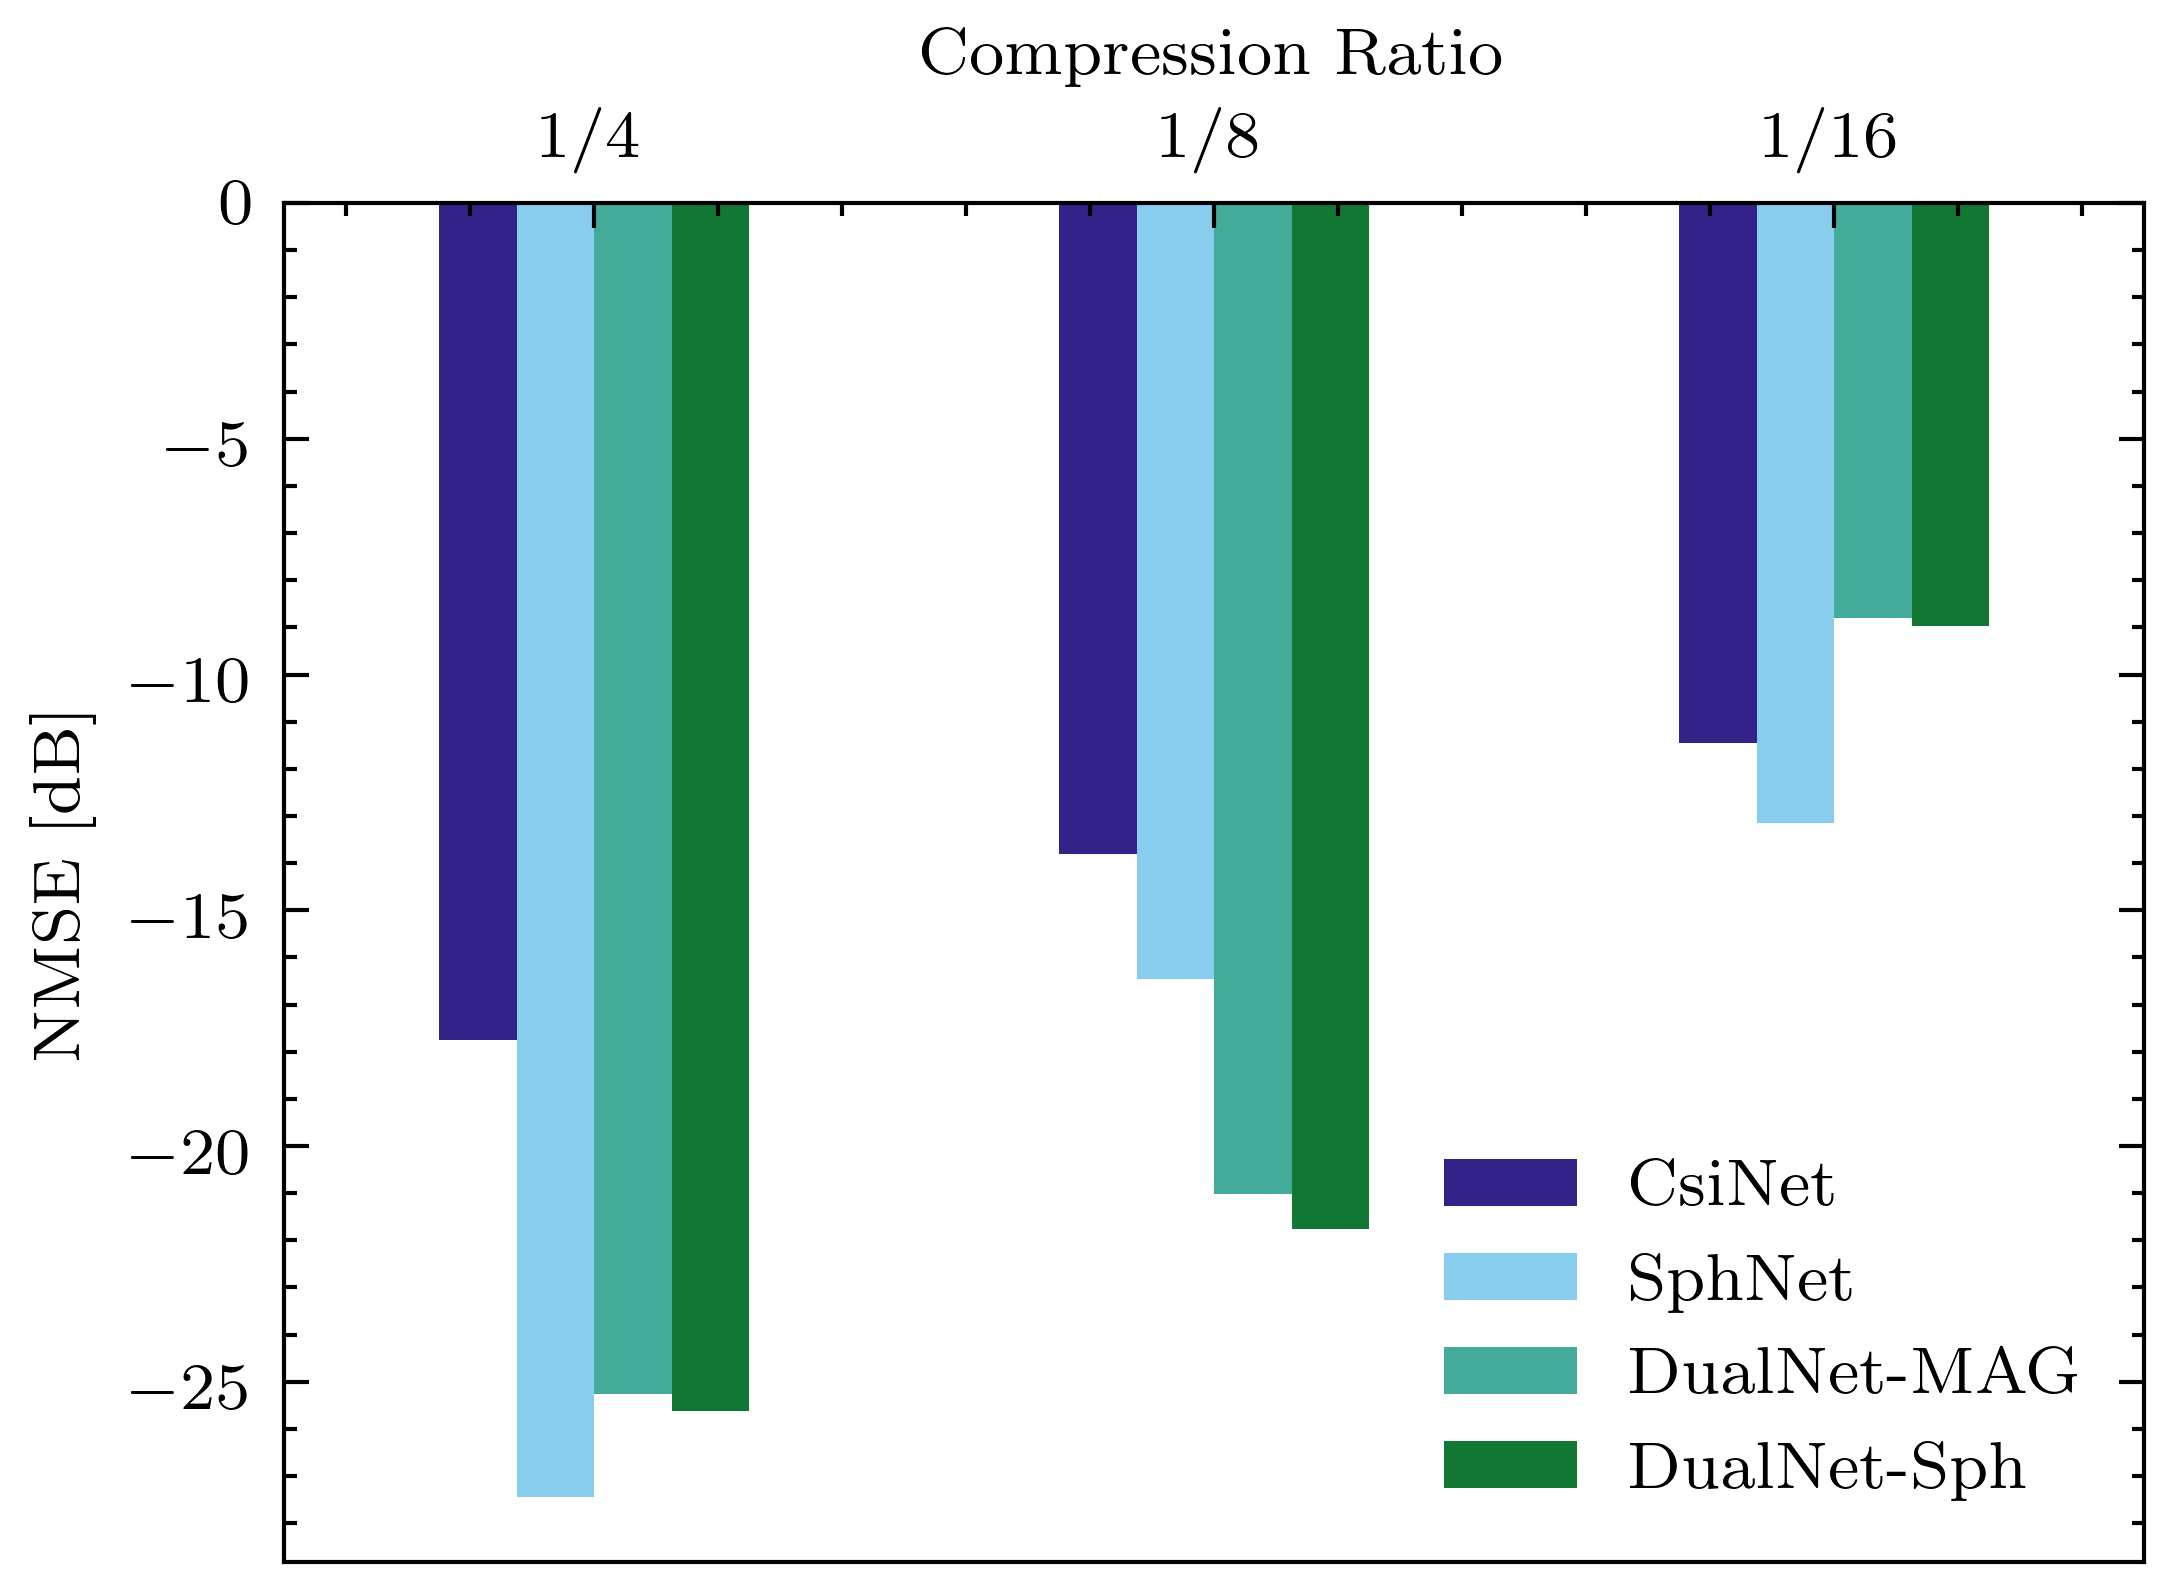
\includegraphics[width=0.47\textwidth]{indoor_res.png}
      } 
      \subfigure[Outdoor] { \label{fignmse_mag:b} 
      % 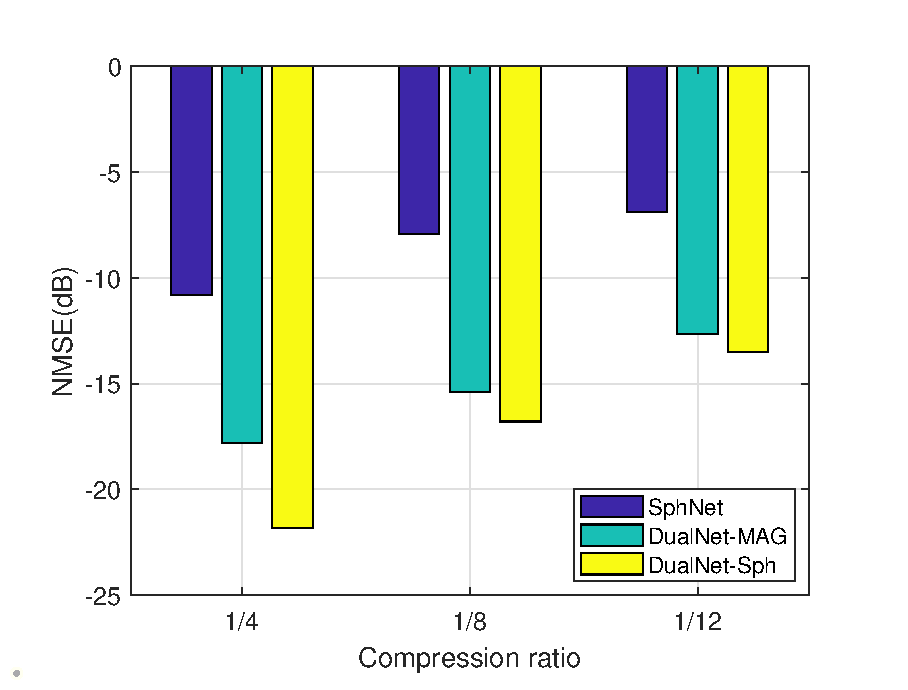
\includegraphics[width=0.46\textwidth]{images/nmse_outdoor_mag.eps} 
      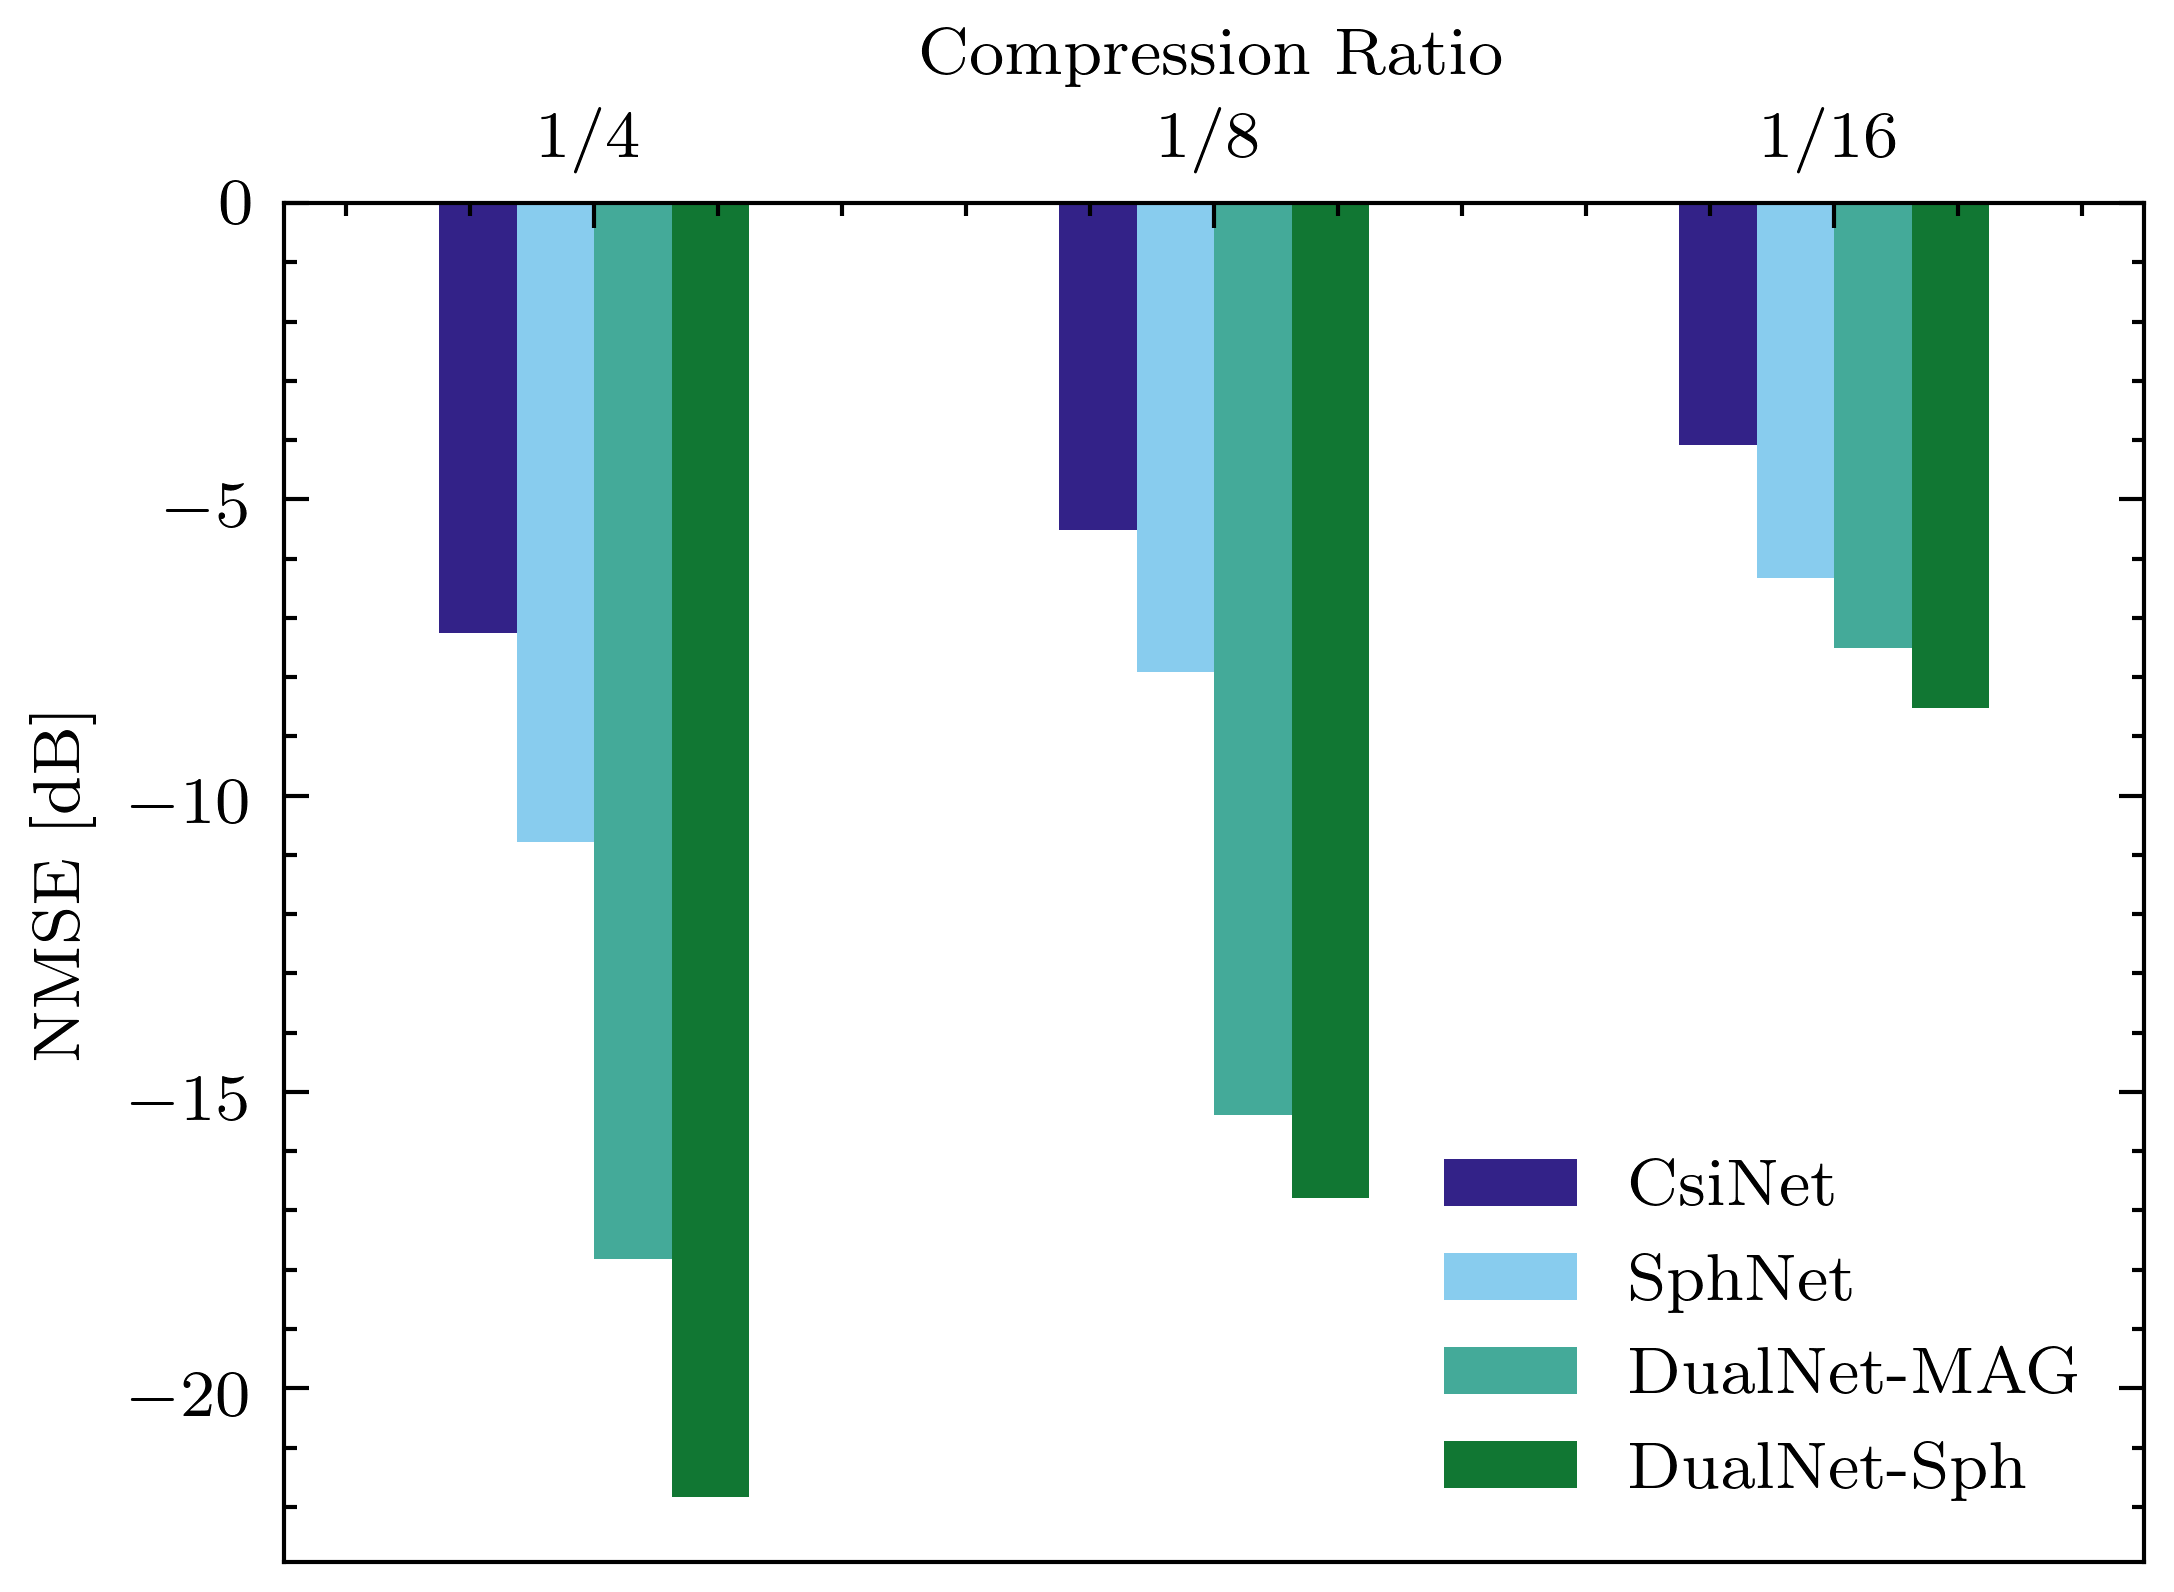
\includegraphics[width=0.47\textwidth]{outdoor_res.png}
      } 
      \caption{NMSE (lower is better) comparison of bidirectional reciprocity and spherical normalization against CsiNet for increasing compression ratio \cite{ref:liu2020sphnet}} 
      \label{fignmse_mag} \vspace*{-2mm}
    \end{figure}
    \blfootnote{\bibentry{ref:liu2020sphnet}}
  \end{frame}
  }

\section{MarkovNet}

  % MarkovNet section frame 
  \begin{frame}[plain]
    \vfill
    \centering
    \begin{beamercolorbox}[sep=8pt,center,shadow=true,rounded=true]{MarkovNet}
      \usebeamerfont{title}\insertsectionhead\par%
      \color{davisblue}\noindent\rule{10cm}{1pt} \\
      \footnotesize{A deep differential autoencoder for efficient temporal learning.}
      % \LARGE{\faFileTextO}
    \end{beamercolorbox}
    \vfill
  \end{frame}

  \begin{frame}{Temporal Correlation}
    CSI estimation techniques benefit from temporal information.
    \begin{figure}[!hbtp] \centering 
      \subfigure[Indoor] {\label{fig:entropy_in} 
      % 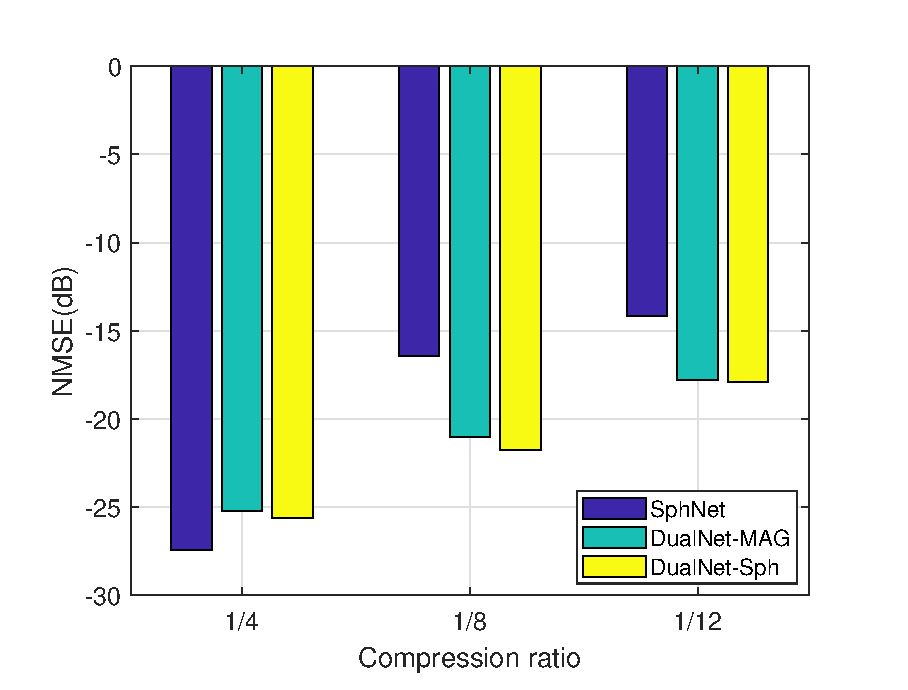
\includegraphics[width=0.46\textwidth]{images/nmse_indoor_mag.eps}
      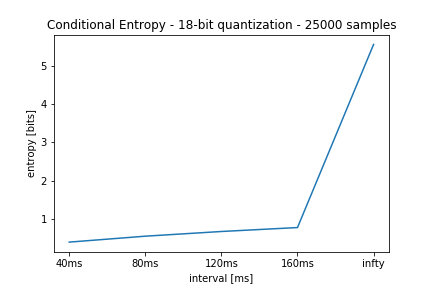
\includegraphics[width=0.47\textwidth]{indoor_entropy.png}
      } 
      \subfigure[Outdoor] { \label{fig:entropy_out} 
      % 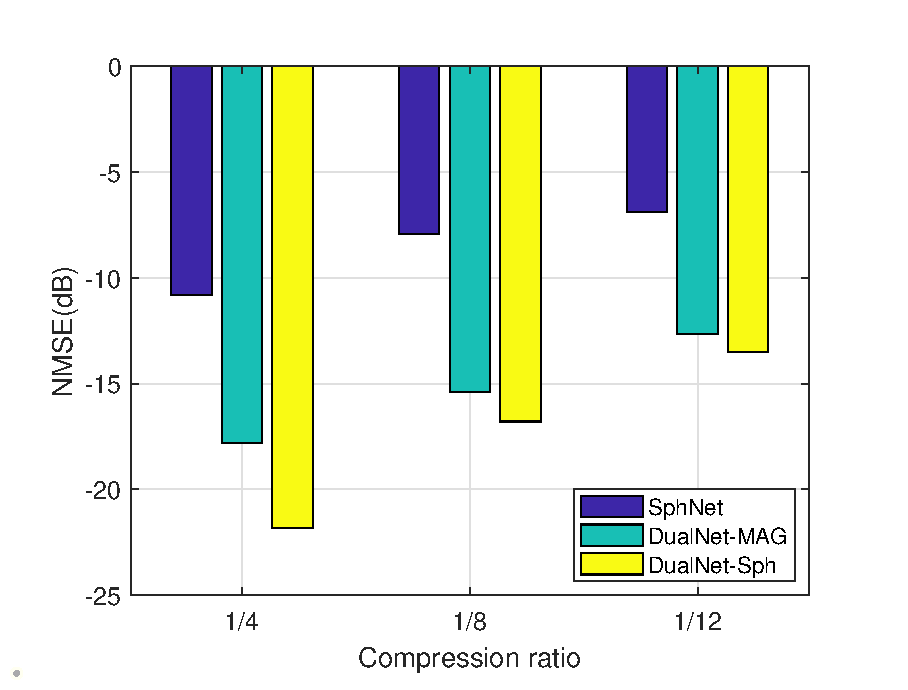
\includegraphics[width=0.46\textwidth]{images/nmse_outdoor_mag.eps} 
      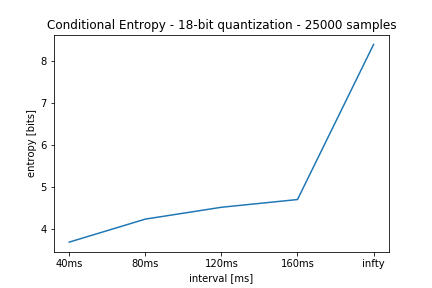
\includegraphics[width=0.47\textwidth]{outdoor_entropy.png}
      } 
      \caption{Conditional entropy between CSI matrices for different feedback intervals. COST2100 model used for (a) Indoor and (b) Outdoor network} 
      \label{fig:entropy} \vspace*{-2mm}
    \end{figure}
  \end{frame}

  \nofoot{
  \begin{frame}{Recurrent Neural Networks for Temporal Correlation}
    \footnotesize{
    Recurrent neural networks (RNNs) contain trainable long short-term memory (LSTM) cells which learn temporal relationships. 
    \begin{figure}[htb] \centering 
      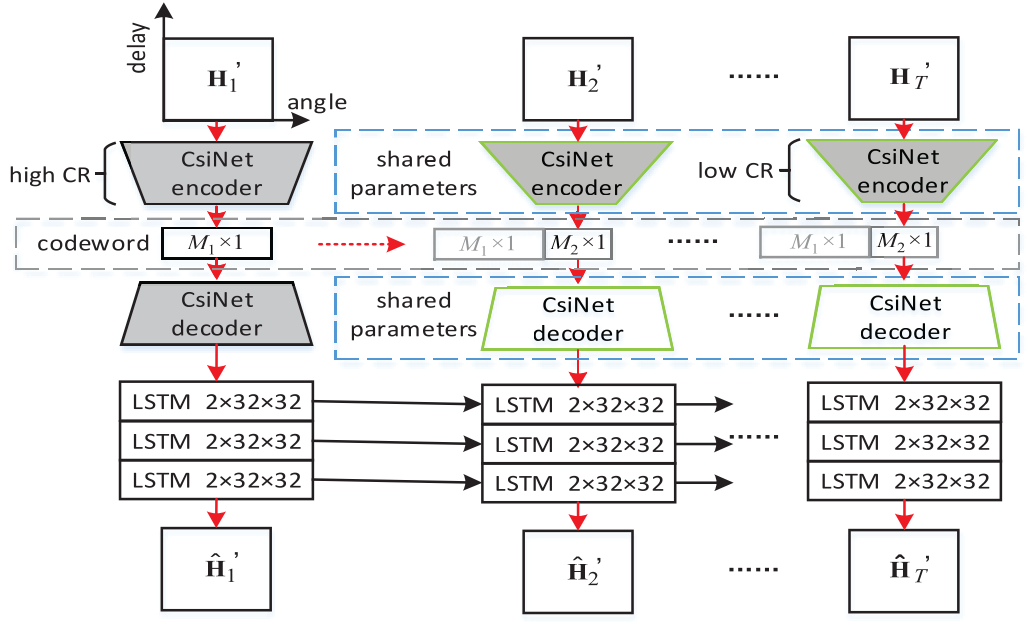
\includegraphics[width=0.6\linewidth]{csinet-lstm.png}
      \caption{CsiNet-LSTM network architecture \cite{ref:Wang2019CsiNetLSTM}.} 
      \label{fig:csinet-lstm} 
    \end{figure}
    }
    \blfootnote{\bibentry{ref:Wang2019CsiNetLSTM}}
  \end{frame}
  }


  \nofoot{
  \begin{frame}{Recurrent Neural Networks for Temporal Correlation}
    % \footnotesize{
    The number of parameters/FLOPs for RNNs is large.
    \begin{table}[htb]
      % \renewcommand{\arraystretch}{1.5}
      \begin{center}
        \caption{Model size and computational complexity of CsiNet-LSTM and CsiNet. M: million.}
        \label{tab:comp-complex-lstm-only} 
        \begin{tabular}{|c|c|c|c|c|}
        \hline
                    & \multicolumn{2}{c|}{\textbf{Parameters}} & \multicolumn{2}{c|}{\textbf{FLOPs}} \\ \hline 
        \textbf{CR} & \textbf{CsiNet-LSTM} & \textbf{CsiNet} & \textbf{CsiNet-LSTM} & \textbf{CsiNet} \\ \hline
        $1/4$       & 132.7 M        & 2.1 M        & 412.9 M        & 7.8 M              \\ \hline
        $1/8$       & 123.2 M        & 1.1 M        & 410.8 M        & 5.7 M              \\ \hline
        $1/16$      & 118.5 M        & 0.5 M        & 409.8 M        & 4.7 M              \\ \hline
        $1/32$      & 116.1 M        & 0.3 M        & 409.2 M        & 4.1 M              \\ \hline
        $1/64$      & 115.0 M        & 0.1 M        & 409.0 M        & 3.9 M              \\ \hline
        \end{tabular}
      \end{center}
    \end{table}
    \blfootnote{\bibentry{ref:Wang2019CsiNetLSTM}}
  \end{frame}
  % }
  }
% {}
  \subsection{Differential Encoding}
% {}
  \nofoot{
  \begin{frame}{MarkovNet: Markov Assumption}
    Instead of learning a temporal dependency
    across multiple timeslots, we proposed a one-step differential encoder.

    For short enough time intervals between $t$ and $t-1$, 
    % CSI data are stationary, i.e. 
    we view CSI data as a Markov chain, i.e.
    \begin{align*} 
      \mathbf H_t &= \gamma\mathbf H_{t-1} + \mathbf V_t,
    \end{align*}
    with $\gamma \in \mathbb R^+$ and i.i.d $\mathbf
    V_t$ such that $\mathbf V_t \sim \mathcal{CN}(\mathbf 0,\Sigma_V)$.
    % $\mathbb E\left[\mathbf V_t\right] = \mathbf 0$.
    \blfootnote{\bibentry{ref:Liu2020MarkovNet}}
  \end{frame}
  }

  \begin{frame}{MarkovNet}
    The ordinary least-squares solution, $\gamma$, is given as
    \begin{align*}
      \gamma &= \frac{\text{Trace}(\mathbb E\left[\mathbf H_{t-1}^H\mathbf H_{t}\right])}{\mathbb E\Arrowvert\mathbf H_t^H \mathbf H_t\Arrowvert^2}.
    \end{align*}
    We utilize the estimator, $\hat \gamma$, based on the second-order statistics of the CSI matrices,
    \begin{align*}
      \hat \gamma &= \frac{\sum_{i=1}^N\text{Trace}(\left[\mathbf H_{t-1}^H(i)\mathbf H_{t}(i)\right])}{\sum_{i=1}^N\Arrowvert\mathbf H_t^H(i) \mathbf H_t(i)\Arrowvert^2},
    \end{align*}
    for training set of size $N$.
  \end{frame}

  \begin{frame}{MarkovNet}
    With the one-step estimator $\hat\gamma$, we propose train an encoder for the estimation error as
    \begin{align*}
      \mathbf s_t &= f_{e,t} (\mathbf H_t - \hat \gamma \hat {\mathbf H}_{t-1}),
    \end{align*}
    and we jointly train a decoder,
    \begin{align*}
      \hat{\mathbf H}_t &= f_{d,t}(\mathbf s_t) + \hat\gamma\hat{\mathbf H}_{t-1}
    \end{align*}
  \end{frame}

  \begin{frame}{MarkovNet: Deep Differential Encoding}
    \begin{figure}[!hbtp]
    \centering
    {
      \fontsize{4pt}{6pt}
      \def\svgwidth{0.8\columnwidth}
      \input{../images/markovnet_schematic.pdf_tex}
    }
    \caption{Abstract architecture for MarkovNet. Networks at $t \geq 2$ are trained to predict the estimation error, $\mathbf E_t$.}
    \label{fig:markovnet_schema}
    \end{figure}
  \end{frame}

  \begin{frame}{MarkovNet: Results ($\text{NMSE}_{\text{truncated}}$)}
    \begin{figure}[!hbtp] \centering 
      \subfigure[Indoor] {\label{fig:diffnet_indoor} 
      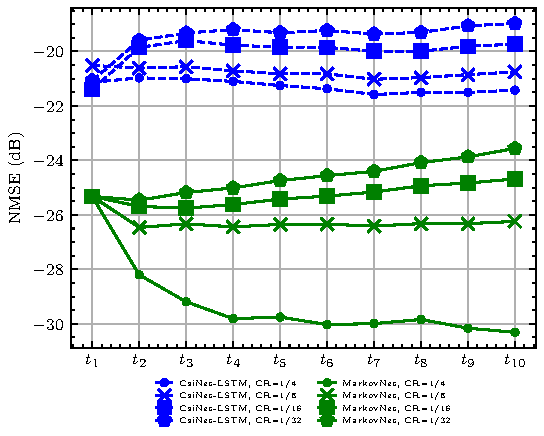
\includegraphics[width=0.46\textwidth]{MarkovNet_truncated_Indoor_10slots.pdf}
      } 
      \subfigure[Outdoor] { \label{fig:diffnet_outdoor} 
      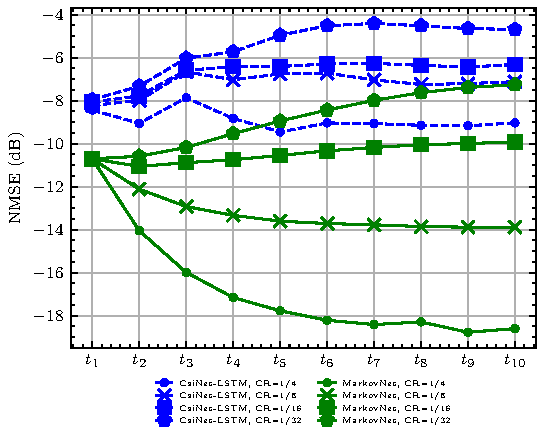
\includegraphics[width=0.46\textwidth]{MarkovNet_truncated_Outdoor_10slots.pdf} 
      } 
      \vspace*{-3mm}

      \caption{$\text{NMSE}_{\text{truncated}}$ comparison of MarkovNet and CsiNet-LSTM 
      at various compression ratios (CR).} 
      \label{fig:diffnet_result} \vspace*{-2mm}
    \end{figure}  
  \end{frame}

  \begin{frame}{MarkovNet: Results ($\text{NMSE}_{\text{all}}$)}
    \begin{figure}[!hbtp] \centering 
      \subfigure[Indoor] {\label{fig:diffnet_indoor} 
      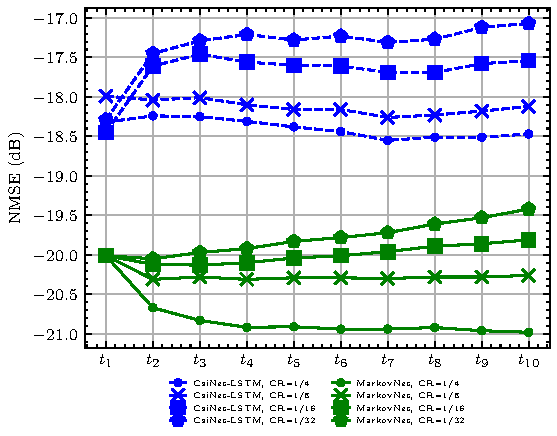
\includegraphics[width=0.46\textwidth]{MarkovNet_Indoor_10slots.pdf}
      } 
      \subfigure[Outdoor] { \label{fig:diffnet_outdoor } 
      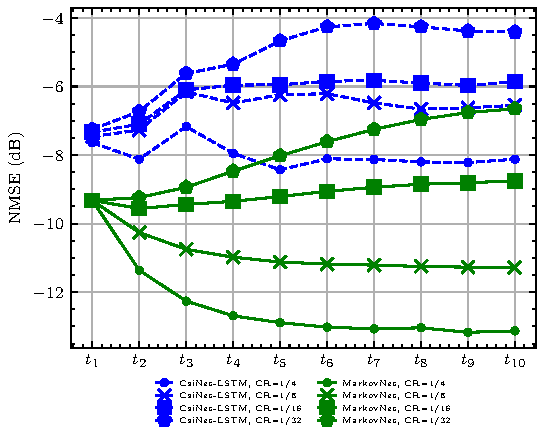
\includegraphics[width=0.46\textwidth]{MarkovNet_Outdoor_10slots.pdf} 
      } 
      \vspace*{-3mm}
      \caption{$\text{NMSE}_{\text{all}}$ comparison of MarkovNet and CsiNet-LSTM 
      at various compression ratios (CR).} 
      \label{fig:diffnet_result} \vspace*{-2mm}
    \end{figure}  
  \end{frame}


  \begin{frame}{MarkovNet: Results}
    \begin{figure}[htb] \centering 
      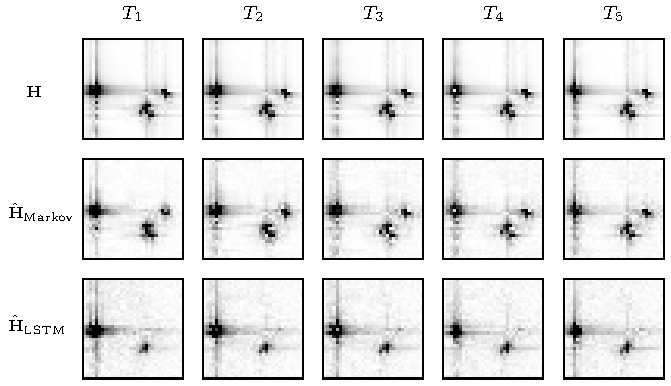
\includegraphics[width=0.9\linewidth]{batch0_csi_compare_cr512.pdf}
      \caption{Ground truth CSI ($\mathbf H$), MarkovNet estimates ($\hat{\mathbf H}_{\text{Markov}}$), and CsiNet-LSTM estimates ($\hat{\mathbf H}_{\text{LSTM}}$) for five timeslots ($T_1$ through $T_5$) on one outdoor sample from the test set (both networks at $\text{CR}=\frac 14$).} 
      \label{fig:csi_img_compare} 
    \end{figure}
  \end{frame}

\section{SphNet-Quant}

  % Background section frame 
  \begin{frame}[plain]
    \vfill
    \centering
    \begin{beamercolorbox}[sep=8pt,center,shadow=true,rounded=true]{SphNet-Quant}
      \usebeamerfont{title}\insertsectionhead\par%
      \color{davisblue}\noindent\rule{10cm}{1pt} \\
      \footnotesize{An end-to-end trained autoencoder with learned feedback quantization.} 
      % \LARGE{\faFileTextO}
    \end{beamercolorbox}
    \vfill
  \end{frame}

  \begin{frame}{SHVQ for CSI Estimation}
    \begin{figure}[!hbtp]
    \centering
    {
      \fontsize{6pt}{8pt}
      \def\svgwidth{0.8\columnwidth}
      \input{../images/csinet_quant.pdf_tex}
    }
    \caption{Abstract architecture for CsiNet-Quant. SoftQuantize layer ($Q(\tilde{\mathbf Z})$) is a continuous, softmax-based relaxation of a $d$-dimensional quantization of the latent layer $\mathbf Z$.}
    \label{fig:csinet_quant}
    \end{figure}
  \end{frame}

  \begin{frame}{Soft Quantization}
    Define the $m$-dimensional codebook of size $L$ as $\mathbf C \in \mathbb R^{m\times L}$. The soft assignments of the $j$-th latent vector $\tilde{\mathbf z}_j$ can be written as,
    \begin{align}
    \phi(\tilde{\mathbf z}_j) &= \left[\frac{\text{exp}(-\sigma \Arrowvert \tilde{\mathbf z}_j - \mathbf c_\ell\Arrowvert^2)}{\sum_{i=1}^L\text{exp}(-\sigma \Arrowvert \tilde{\mathbf z}_j - \mathbf c_i\Arrowvert^2)}\right]_{\ell\in [L]} \in \mathbb R^L, \label{eq:soft_assign}
    \end{align}

    which is referred to as the `softmax' function. $\sigma$ is a \emph{temperature} or \emph{annealing} parameter which controls the degree of quantization,
    \begin{align}
      \lim_{\sigma \to \infty} \phi(\tilde{\mathbf z}_j) &= \text{onehot}(\tilde{\mathbf z}_j) = \begin{cases} 1 & \ell = \underset{\ell}{\text{argmax}} \; \phi(\tilde{\mathbf z}_j)[\ell] \\ 0 & \text{otherwise} \end{cases}
    \end{align}
    % TODO: visualize this using the inkscape diagram?
  \end{frame}

  \begin{frame}{Latent Entropy Estimation}
    \footnotesize{
    The soft assignments $\phi$ admit probability masses over the codewords,
    \begin{align*} 
      q_j = \phi(\tilde{\mathbf z}).
    \end{align*}
    Based on finite samples, we define the histogram probability estimates $p_j$
    \begin{align*}
    p_j &= \frac{|\{e_l(\mathbf z_i)|l\in[m], i \in [N], e_l(\mathbf z_i)=j\}|}{mN}.
    \end{align*}
    Our target for the rate loss is the crossentropy between $p_j$ and $q_j$ term,
    \begin{align*}
    H(\phi) := H(p,q) &= -\sum_{j=1}^L p_j\log q_j = H(p) + D_{\text{KL}}(p\Arrowvert q).
    \end{align*}
    }
  \end{frame}

  \begin{frame}{Rate-Distortion Loss}
    \footnotesize{
    Loss function for soft quantization $=$ regularized rate-distortion function.
    \begin{align}
      \underset{\theta_e, \theta_d, \mathbf C}{\text{argmin}}\; L_{d}(\mathbf H, \hat {\mathbf H}) + \lambda L_{\ell^2}(\theta_e, \theta_d, \mathbf C) + \beta L_{r}(\theta_e,\mathbf C)
    \end{align} 
    Where the different loss terms are

      \begin{table}[]
      \centering
      % \caption{Parameters used for COST2100 simulations for both Indoor and Outdoor datasets.}
      % \label{tab:cost-params}
      \begin{tabular}{c|c|l}
      \toprule
      \textbf{Term} & \textbf{Definition} & \textbf{Description} \\ \midrule
       $ L_{d}(\mathbf H, \hat {\mathbf H}) $ & $ \frac 1N \sum_{i=1}^N\Arrowvert \mathbf H_i - g(Q(f(\mathbf H_i, \theta_e), \mathbf C), \theta_d) \Arrowvert^2 $ & distortion loss \\ \hline
       $ L_{\ell^2}(\theta_e, \theta_d, \mathbf C) $ & $ \Arrowvert\theta_e\Arrowvert^2+\Arrowvert\theta_d\Arrowvert^2+\Arrowvert \mathbf C \Arrowvert^2 $ & $\ell^2$ penalty \\ \hline
       $ L_{r}(\theta_e, \mathbf C) $ & $m\beta H(\phi)$  & rate loss \\ \bottomrule
      \end{tabular}
      \end{table}
    }
  \end{frame}
% {}

\subsection{Results}

  \nofoot{
  \begin{frame}{Results: Rate-Distortion (Outdoor)}
    \begin{figure}[htb] \centering 
      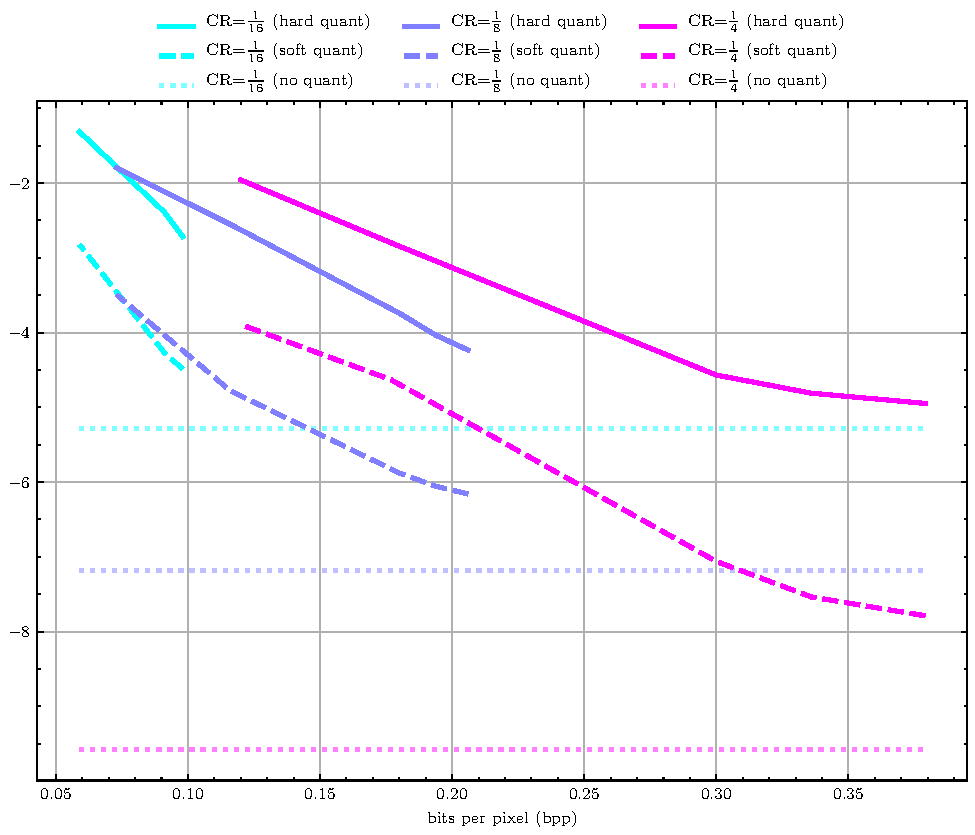
\includegraphics[width=0.7\linewidth]{rate-distortion-all-cr-H4.pdf}
      \caption{Rate distortion of CsiNet-Quant under minmax normalization using: $L=1024$ centers, $d=4$.} 
     \label{fig:rate-distortion-minmax} 
    \end{figure}
  \end{frame}
  }

  \nofoot{
  \begin{frame}{Results: Rate-Distortion (Outdoor)}
    \begin{figure}[htb] \centering 
      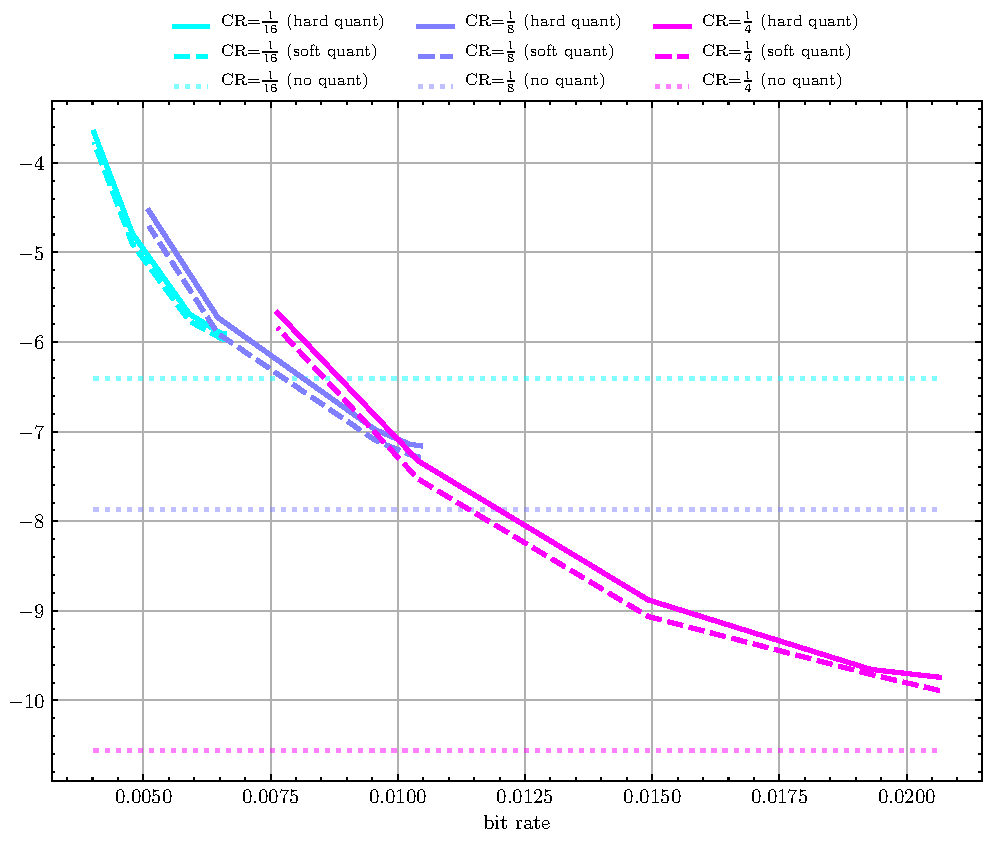
\includegraphics[width=0.7\linewidth]{bitrate-distortion-all-cr-sphH4-K100-outdoor.pdf}
      % 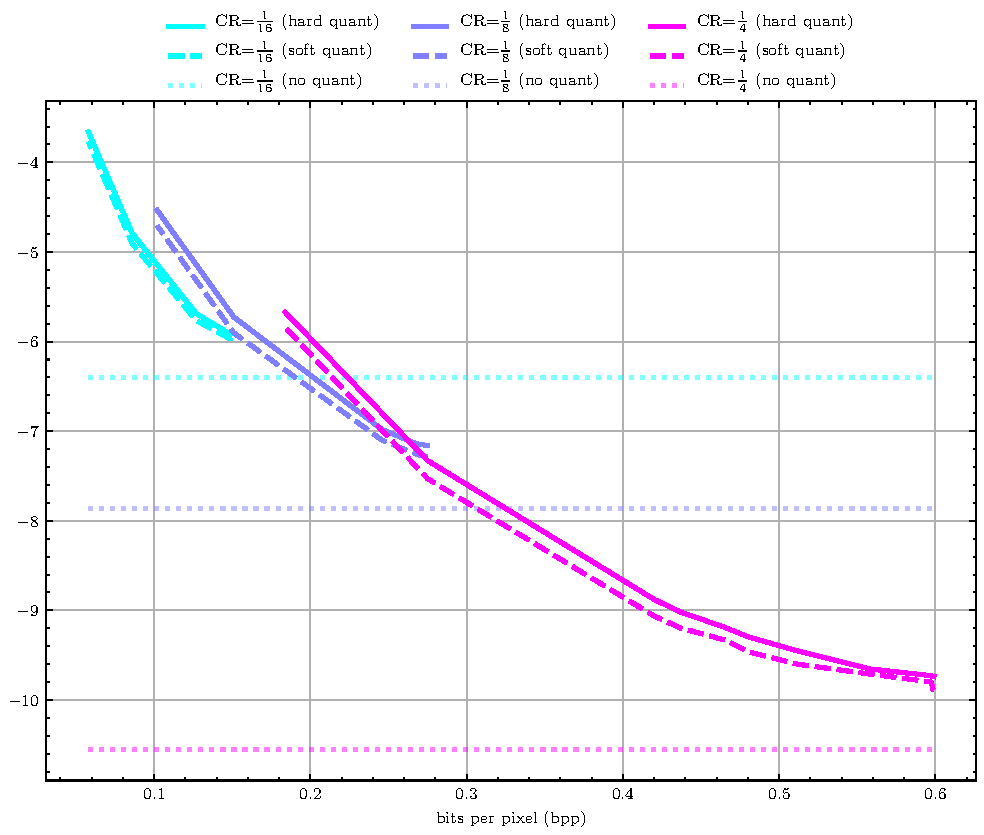
\includegraphics[width=0.7\linewidth]{rate-distortion-all-cr.pdf}
      \caption{Rate distortion of SphNet-Quant using: $L=1024$ centers, CR$=\frac 14$, $d=4$. Bit rates are realized under arithmetic coding of quantized features.} 
      \label{fig:rate-distortion} 
    \end{figure}
  \end{frame}
  }

  \nofoot{
  \begin{frame}{Results: Rate-Distortion (Outdoor)}
    \begin{figure}[htb] \centering 
      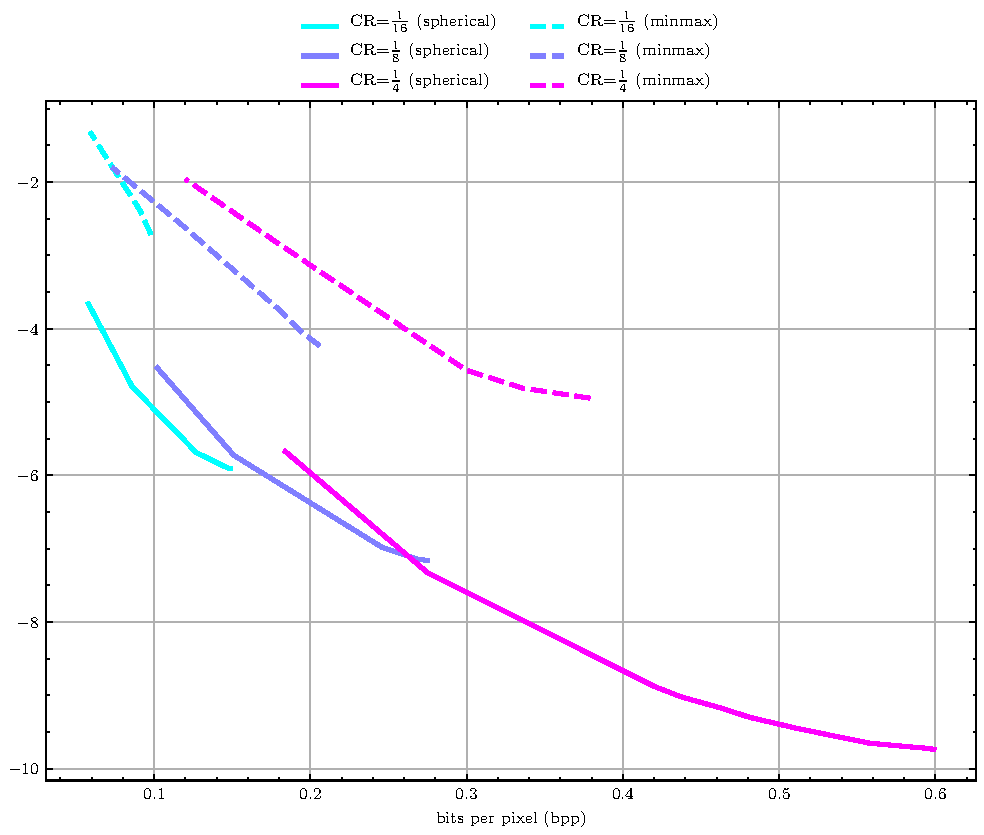
\includegraphics[width=0.7\linewidth]{rate-distortion-all-norm.pdf}
      \caption{Rate distortion of CsiNet-Quant under both minmax (dotted line) and spherical (solid line) normalization using: $L=1024$ centers, $d=4$. Hard quantization performance shown for each CR.} 
      \label{fig:rate-distortion-norms} 
    \end{figure}
  \end{frame}
  }


\section*{Questions?}
    \begin{frame}[plain]
        \vfill
      \centering
      \begin{beamercolorbox}[sep=8pt,center,shadow=true,rounded=true]{title}
        \usebeamerfont{title}\insertsectionhead\par%
        \small{\url{mdelrosa@ucdavis.edu}}
        \color{davisblue}\noindent\rule{10cm}{1pt} \\
        % \LARGE{\faFileTextO}
      \end{beamercolorbox}
      \vfill
    \end{frame}

\section*{References}
  \begin{frame}{References}
    % https://latex.org/forum/viewtopic.php?t=12027
    \setbeamertemplate{bibliography item}[text]
    \bibliographystyle{ieeetr}
    \tiny{\bibliography{../cited_works}}
    \tiny{\textdagger $\rightarrow$ equal contribution}
  \end{frame}

\section*{Appendix}

  % Appendix section frame 
  \begin{frame}[plain]
    \vfill
    \centering
    \begin{beamercolorbox}[sep=8pt,center,shadow=true,rounded=true]{Appendix}
      \usebeamerfont{title}\insertsectionhead\par%
      \color{davisblue}\noindent\rule{10cm}{1pt} \\
      % \LARGE{\faFileTextO}
    \end{beamercolorbox}
    \vfill
  \end{frame} 

  \begin{frame}{Multivariate Autoregression (MAR)}
    Rather than scalar $\hat\gamma \in \mathbb R^+$, we can derive a multivariate $p$-step predictor, $\mathbf W_1, \dots, \mathbf W_p$.
    Given $p$ prior CSI samples, the mean-square optimal predictor
    $\hat H_t$ is a linear combination of these the prior CSI samples,
    \begin{equation}
    \mathbf{\hat H}_{t} = \mathbf{H}_{t-1} \mathbf W_{1} + \dots + \mathbf{H}_{t-p} \mathbf W_{p} + \mathbf E_t.
    \end{equation}
  \end{frame}

  \begin{frame}{Multivariate Autoregression (MAR)}
    Error terms are uncorrelated with the CSI samples
    (i.e. $\mathbf H_{t-i}^H \mathbf E_t = 0$ for all $i \in [0, \dots, p]$),
    and we pre-multiply by $\mathbf H_{t-i}^H$,
    \begin{align}
    \mathbf{H}_{t-i}^H\mathbf{\hat H}_{t} &= \mathbf{H}_{t-i}^H\mathbf{H}_{t-1} \mathbf W_{1} + \dots + \mathbf{H}_{t-i}^H\mathbf{H}_{t-p} \mathbf W_{p} + \mathbf{H}_{t-i}^H\mathbf E_t \nonumber \\
                        &= \mathbf{H}_{t-i}^H\mathbf{H}_{t-1} \mathbf W_{1} + \dots + \mathbf{H}_{t-i}^H\mathbf{H}_{t-p} \mathbf W_{p}. \label{eq:var-init}
    \end{align}
  \end{frame}

  \begin{frame}{Multivariate Autoregression (MAR)}
    Denote the correlation matrix 
    $\mathbf R_i = \mathbb E [\mathbf H^H_{t-i}\mathbf H_{t}]$.
    We presume the CSI matrices are generated by a 
    stationary process, and consequently, 
    they have the following properties:
    \begin{enumerate}
      \item $\mathbf R_i = \mathbb E [\mathbf H^H_{t-i}\mathbf H_{t}] = \mathbb E [\mathbf H^H_{t}\mathbf H_{t+i}]$
      \item $\mathbf R_i = \mathbf R^H_{-i}$
    \end{enumerate}
  \end{frame}

  \begin{frame}{Multivariate Autoregression (MAR)}
    Taking the expectation, we can write (\ref{eq:var-init})
    as a linear combination of correlation matrices,
    \begin{align*}
    \mathbf R_{i+1} &= \mathbf{R}_{i} \mathbf W_{1} + \dots + \mathbf{R}_{i-p+1} \mathbf W_{p}. 
    \end{align*}
    For $p$ CSI samples, we can write a system of $p$
    equations, which admits the following,
    \begin{align*}
      \begin{bmatrix}
        \mathbf R_{1} \\ \mathbf R_{2} \\ \dots \\ \mathbf R_{p} \\
      \end{bmatrix}
      &= 
      \begin{bmatrix}
        \mathbf R_{0} & \mathbf R_1^H & \dots  & \mathbf R_{p-1}^H \\
        \mathbf R_{1} & \mathbf R_0   & \dots  & \mathbf R_{p-2}^H \\
        \vdots      &         & \ddots & \vdots \\
        \mathbf R_{p-1} & \mathbf R_{p-2}   & \dots  & \mathbf R_{0} \\
      \end{bmatrix}
      \begin{bmatrix}
        \mathbf W_{1} \\ \mathbf W_{2} \\ \dots \\ \mathbf W_{p} \\
      \end{bmatrix}.
    \end{align*}
  \end{frame}


  \begin{frame}{Multivariate Autoregression (MAR)}
    Solving for the coefficient matrices admits the solution
    \begin{align}
      \begin{bmatrix}
        \mathbf W_{1} \\ \mathbf W_{2} \\ \dots \\ \mathbf W_{p} \\
      \end{bmatrix}
      &= 
      \begin{bmatrix}
        \mathbf R_{0} & \mathbf R_1^H & \dots  & \mathbf R_{p-1}^H \\
        \mathbf R_{1} & \mathbf R_0   & \dots  & \mathbf R_{p-2}^H \\
        \vdots      &         & \ddots & \vdots \\
        \mathbf R_{p-1} & \mathbf R_{p-2}   & \dots  & \mathbf R_{0} \\
      \end{bmatrix}^{+}
      \begin{bmatrix}
        \mathbf R_{1} \\ \mathbf R_{2} \\ \dots \\ \mathbf R_{p} \\
      \end{bmatrix}, \label{eq:mar-solution}
    \end{align}
    where $[\cdot]^+$ denotes the Moore-Penrose pseudoinverse.
  \end{frame}

  \begin{frame}{Differential Entropy Estimation: Multivariate Normal}
    \begin{figure}[htb] \centering 
      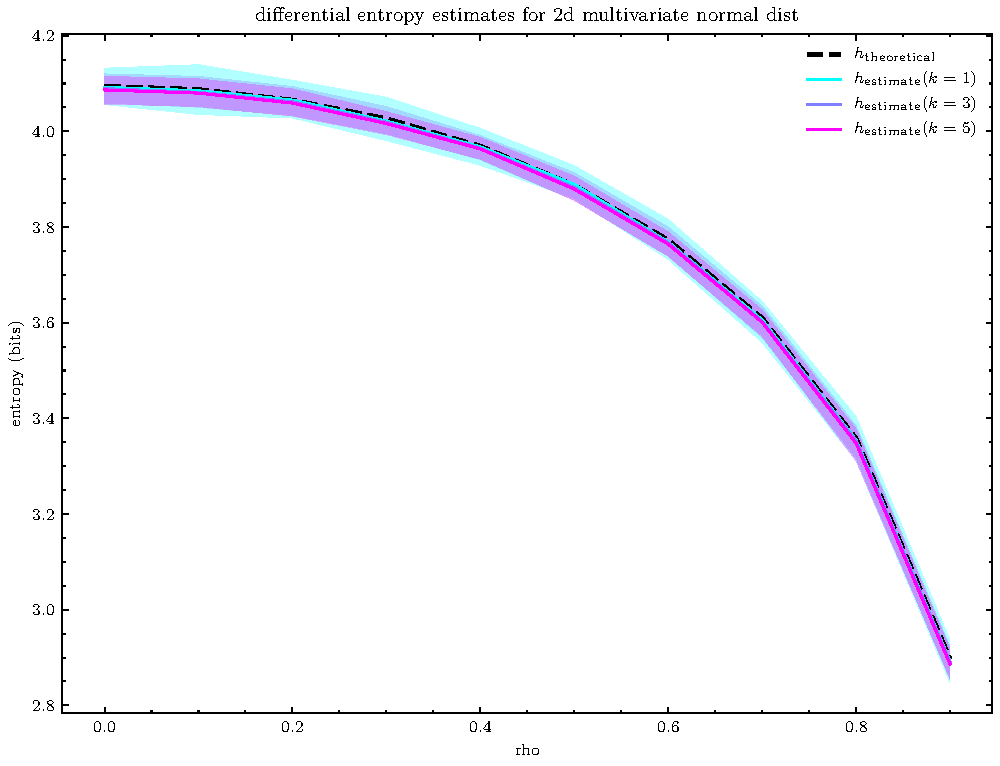
\includegraphics[width=0.7\linewidth]{multivar_normal.pdf}
      \caption{Differential entropy and estimates for 2d multivariate normal distribution. Estimates are based on the KL estimator \cite{ref:Kozachenko1987SampleEstimate} using the NPEET library \cite{ref:VerSteeg2019NPEET}.} 
      \label{fig:multivar-normal-valid} 
    \end{figure}
  \end{frame}


% column example
    % \begin{frame}{CsiNet}
    % \begin{columns}[T] % align columns
    % \begin{column}{.48\textwidth}
    %   \begin{itemize}
    %     \item Autoencoder-based structure for learned CSI compression and feedback \cite{ref:csinet}
    %     \item Expanded their work to use Recurrent Neural Networks \cite{ref:Wang2019CsiNetLSTM}
    %   \end{itemize}
    % \end{column}%
    % \hfill%
    % \begin{column}{.48\textwidth}
    %   \fignocap{0.9}{images/csinet-fig.PNG}
    % \end{column}%
    % \end{columns}
    %   % [3] CsiNet paper
    %   % [4] CsiNet-LSTM paper
    % \end{frame}

\end{document}
